% !TEX root = perelman-geometry.tex
%!TEX TS-program = pdflatex
%!TEX encoding = UTF-8 Unicode



\setchapterpreamble[o]{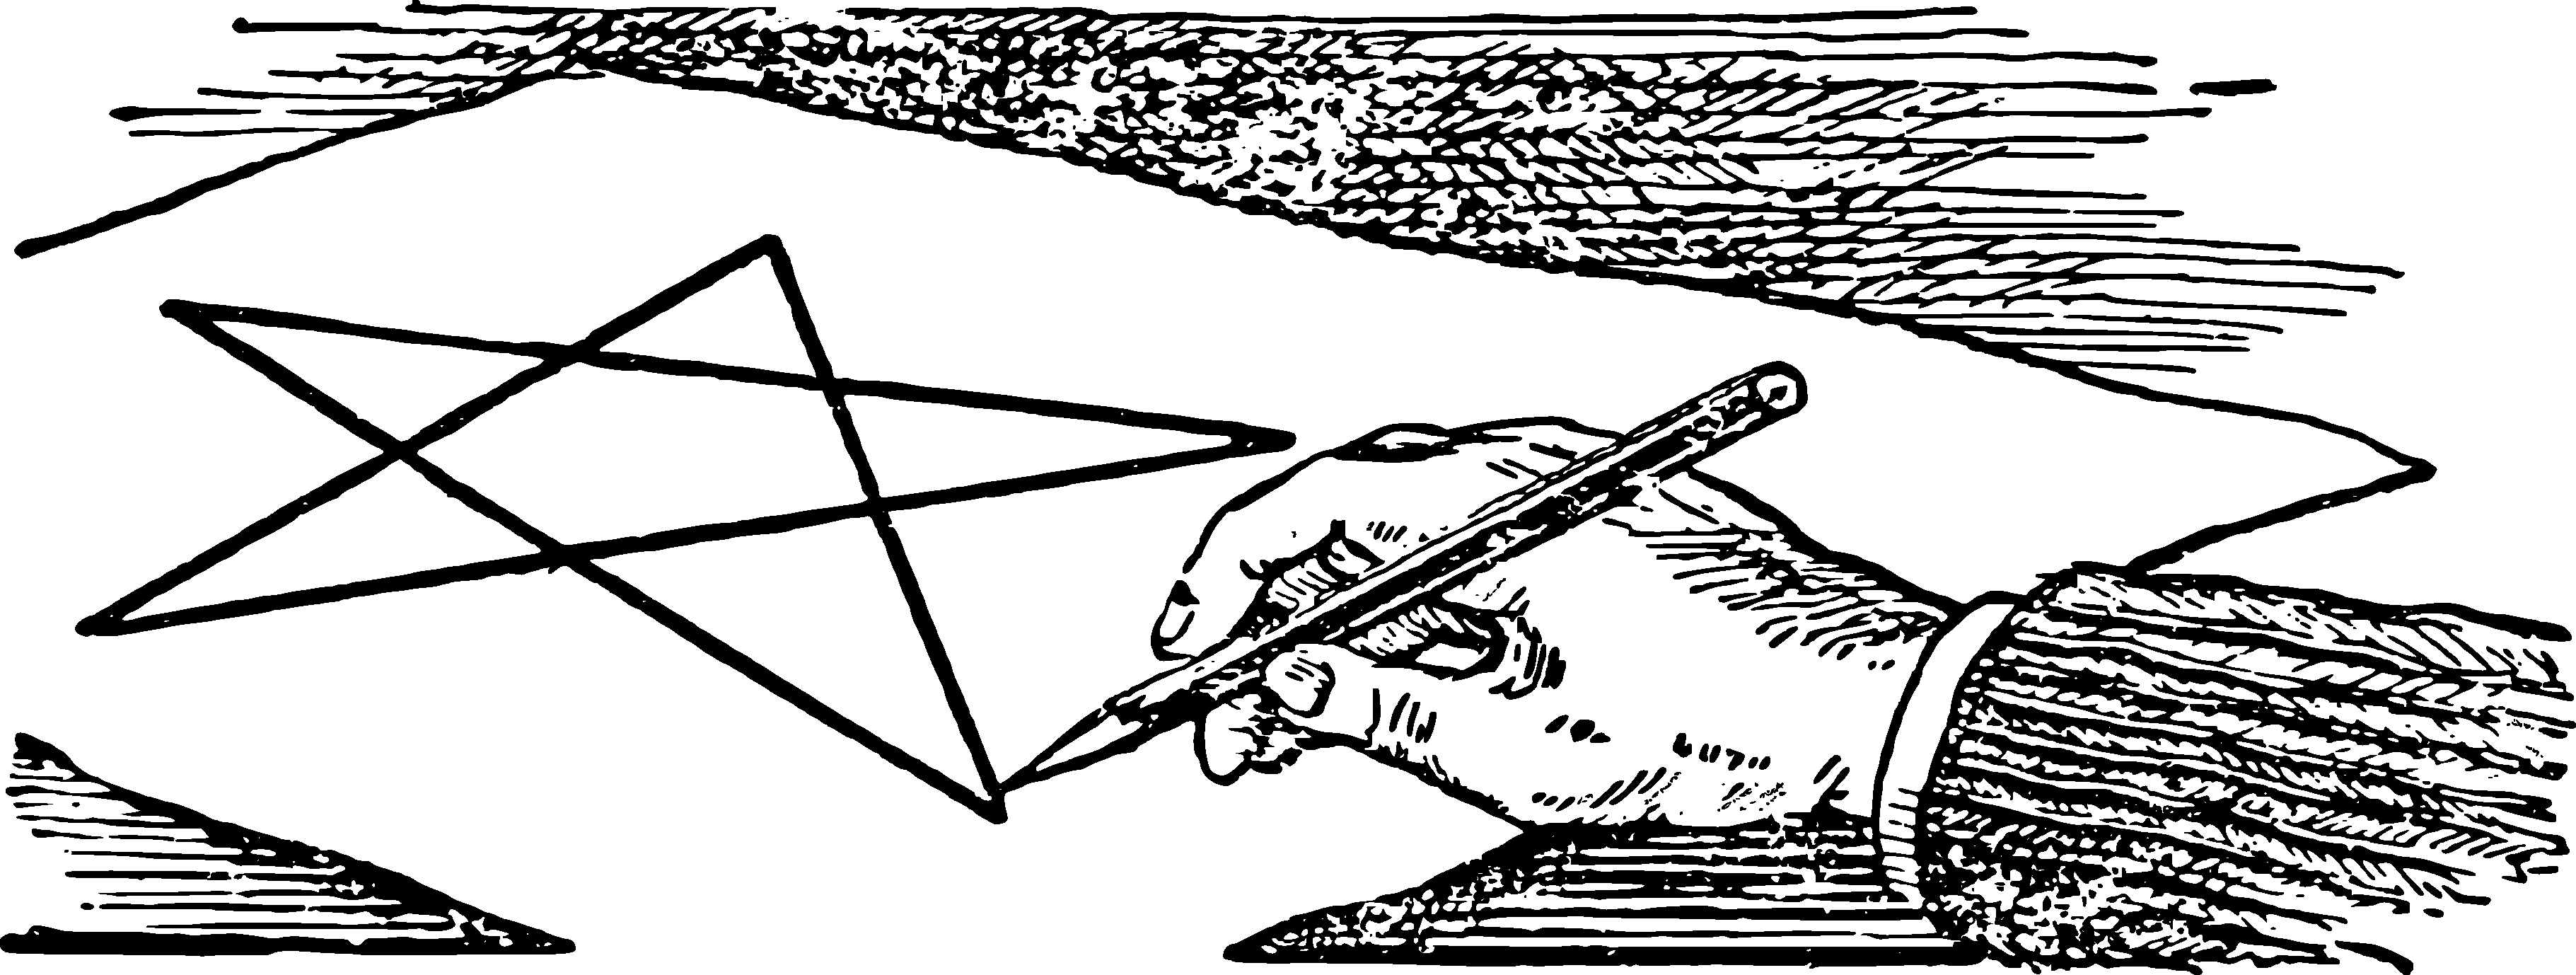
\includegraphics[width=1.2\textwidth]{figures/ch-10/fig-ch-10-head.pdf}\bigskip}

\chapter[Geometry Without Measurements And Calculations]{Geometry Without Measurements And Without Calculations}
\label{ch-10}



\section{Building without a compass}
\label{sec-10.1}

When solving geometric construction problems, rulers and compasses are usually used. However, we will now see that sometimes it is possible to do without a compass in such cases where at first glance it seems absolutely necessary.

\begin{figure}[h!]
\centering
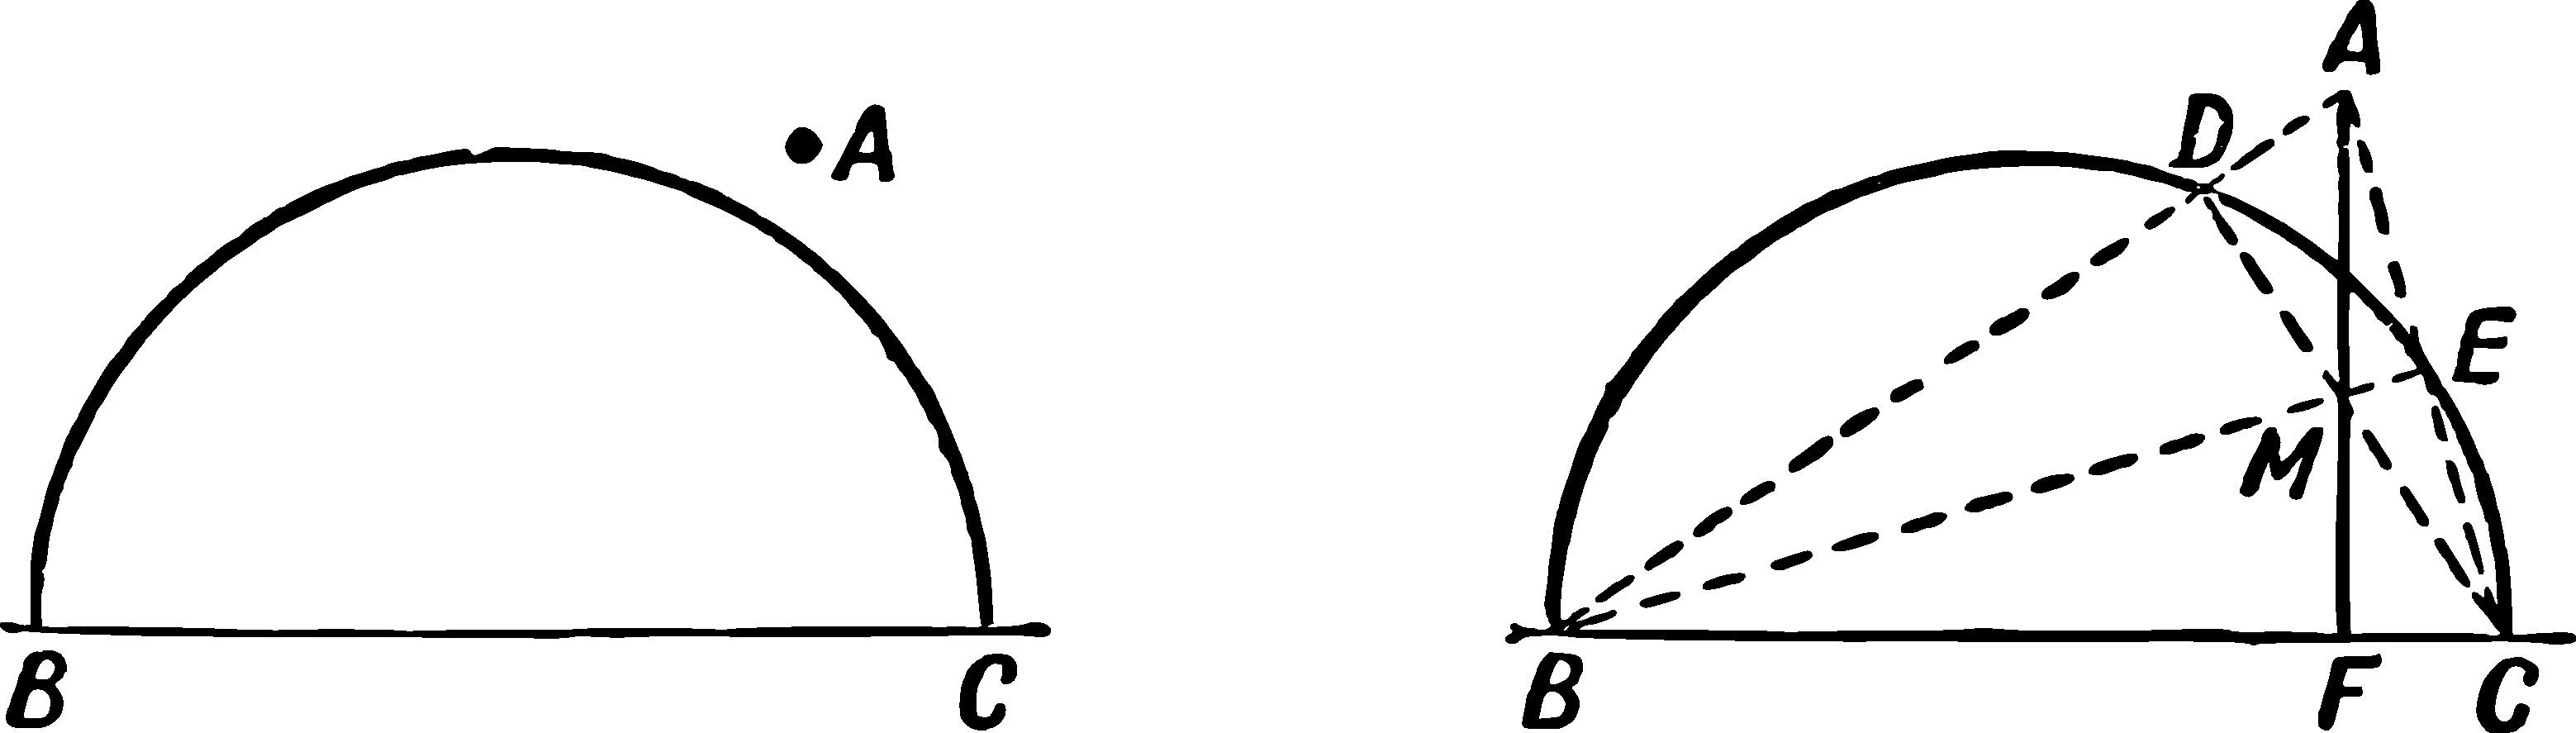
\includegraphics[width=0.9\textwidth]{figures/ch-10/fig-141.pdf}
\sidecaption{The task of building and solving it. The first case.\label{fig-141}}
\end{figure}

\ques From point $A$ (\figr{fig-141}, left), lying outside the given semicircle, drop a perpendicular to its diameter without using a compass. The position of the centre of the semicircle is not indicated.

\ans We will use the property of a triangle that all its altitudes intersect at a single point. Connect $A$ with  $B$ and $C$; we get points $D$ and $E$ (\figr{fig-141}, right). The lines $BE$ and $CD$ are obviously the altitudes of triangle $ABC$. The third altitude, which is the required perpendicular to $BC$, must pass through the intersection point of the other two, i.e., point $M$. By drawing a line through points $A$ and $M$ with a ruler, we meet the requirements of the task without using a compass. 

\begin{figure}[h!]
\centering
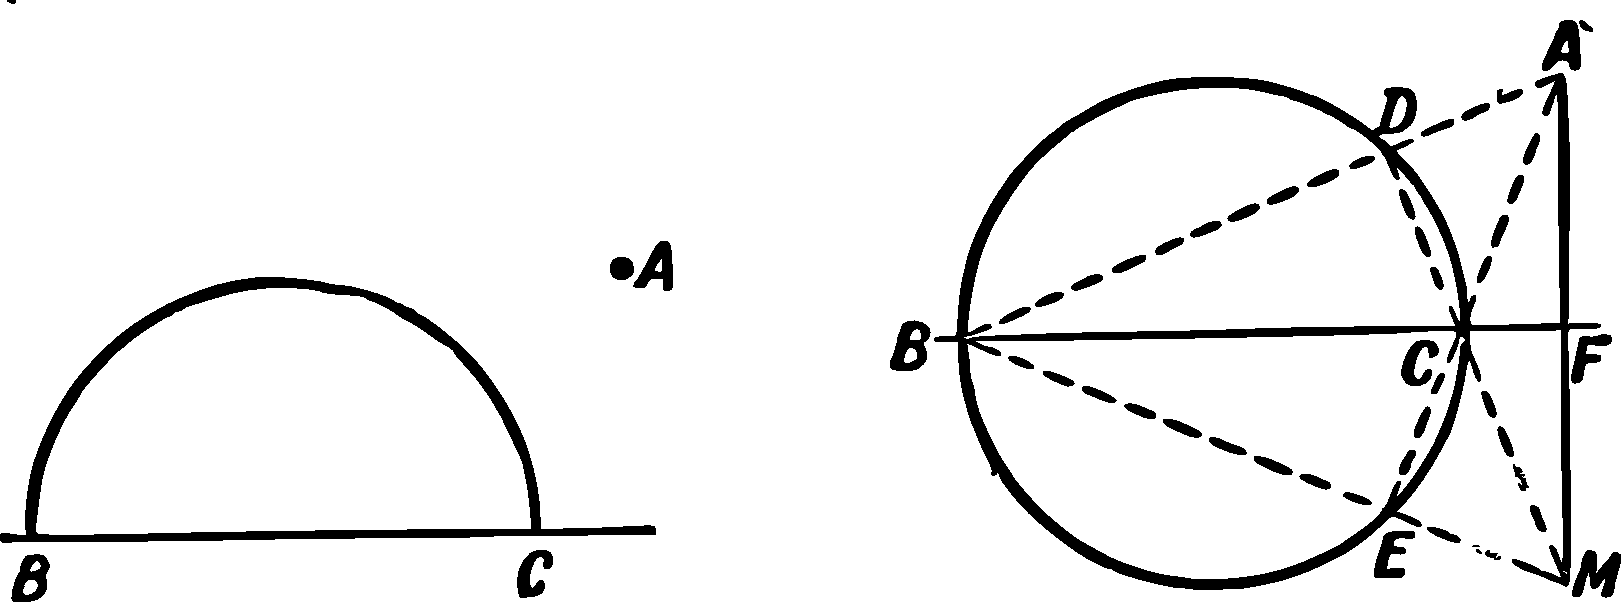
\includegraphics[width=0.9\textwidth]{figures/ch-10/fig-142.pdf}
\sidecaption{The same task. Second case.\label{fig-142}}
\end{figure}


If the point is positioned such that the required perpendicular falls on the extension of the diameter (\figr{fig-142}), then the problem is solvable only if a full circle, rather than a semicircle, is given. \figr{fig-142} shows that the solution is no different from the one we are already familiar with; only the altitudes of triangle $ABC$ intersect not inside, but outside of it.


\section{Centre of Gravity of a Plate}
\label{sec-10.2}

\begin{marginfigure}[-1cm]%[h!]
\centering
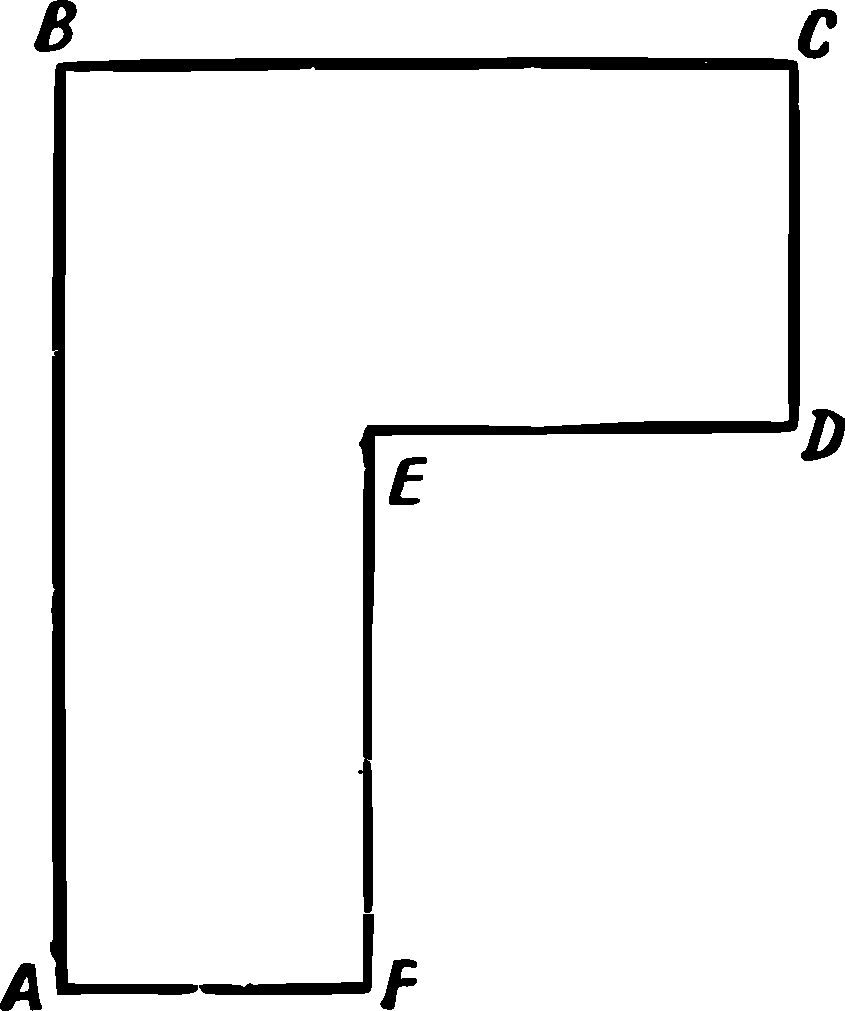
\includegraphics[width=\textwidth]{figures/ch-10/fig-143.pdf}
\sidecaption{Using only a ruler, find the centre of gravity of the depicted plate.\label{fig-143}}
\end{marginfigure}


\ques You probably know that the centre of gravity of a thin, uniform plate, which has the shape of a rectangle or a rhombus, is located at the intersection of the diagonals, and if the plate is triangular, it is at the intersection of the medians. If the plate is circular, it is at the centre of the circle.





Now try to figure out how to find the centre of gravity of a plate made up of two arbitrary rectangles joined into one shape, as shown in \figr{fig-143}. Let's agree to use only a ruler and not to measure or calculate anything.


\ans Extend side $DE$ to intersect with $AB$ at point $N$ and side $FE$ to intersect with $BC$ at point $M$ (\figr{fig-144}). We will first consider the given figure as composed of the rectangles $ANEF$ and $NBCD$. The centre of gravity of each of them is at the intersection points of their diagonals, $O_{1}$ and $O_{2}$.


\begin{marginfigure}%[h!]
\centering
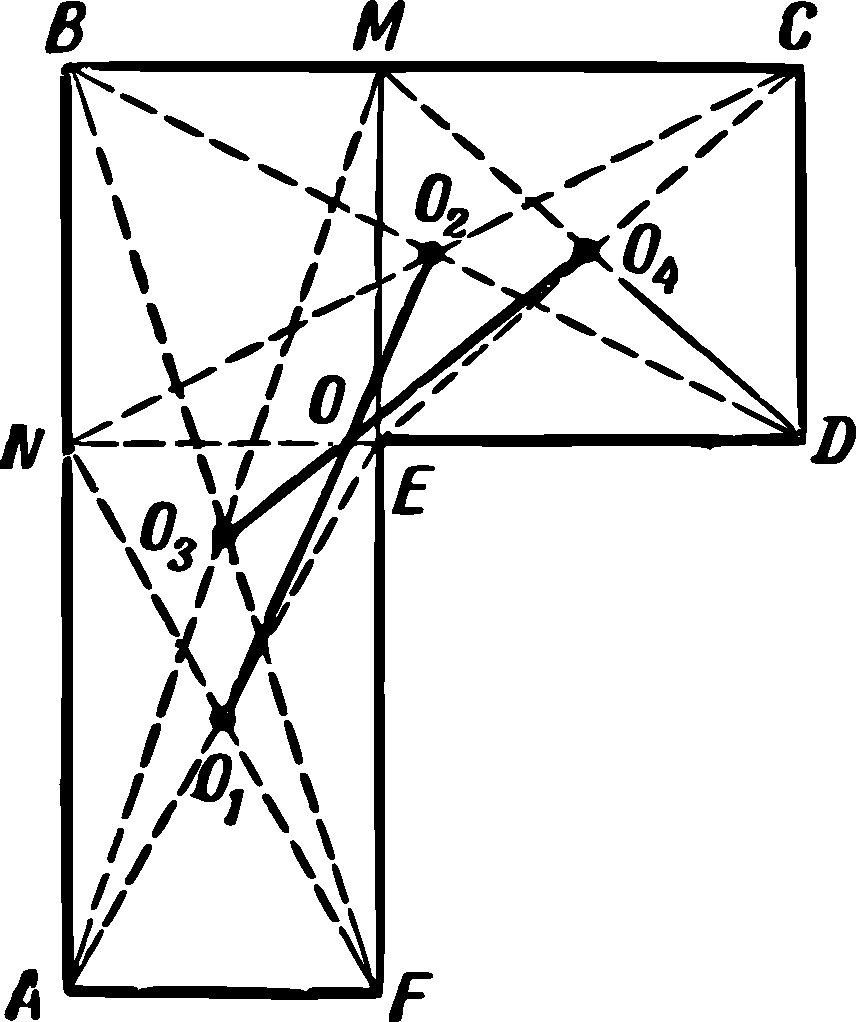
\includegraphics[width=\textwidth]{figures/ch-10/fig-144.pdf}
\sidecaption{The centre of gravity of the plate found.\label{fig-144}}
\end{marginfigure}


Therefore, the centre of gravity of the entire figure lies on the line $O_{1}O_{2}$. Now, consider the same figure as composed of the rectangles $ABMF$ and $EMCD$, whose centres of gravity are at the intersection points of their diagonals, $O_{3}$ and $O_{4}$. The centre of gravity of the entire figure lies on the line $O_{3}O_{4}$. Hence, it lies at the point $O$ where the lines $O_{1}O_{2}$ and $O_{3}O_{4}$ intersect. All these constructions are indeed carried out only with the help of a ruler.






\section{Napoleon's Task}
\label{sec-10.3}


We have just been dealing with a construction performed using only a ruler, without resorting to a compass (on the condition that one circle is given in the drawing in advance). Now let us consider several problems in which the opposite restriction is introduced: the use of a ruler is prohibited, and all constructions must be performed using only a compass. One such problem interested Napoleon (who, as is well known, was interested in mathematics). After reading a book on such constructions by the Italian scientist Mascheroni, he posed the following problem to French mathematicians:

\ques Divide a given circle into four equal parts without using a ruler. The position of the centre of the circle is given.


\begin{marginfigure}%[h!]
\centering
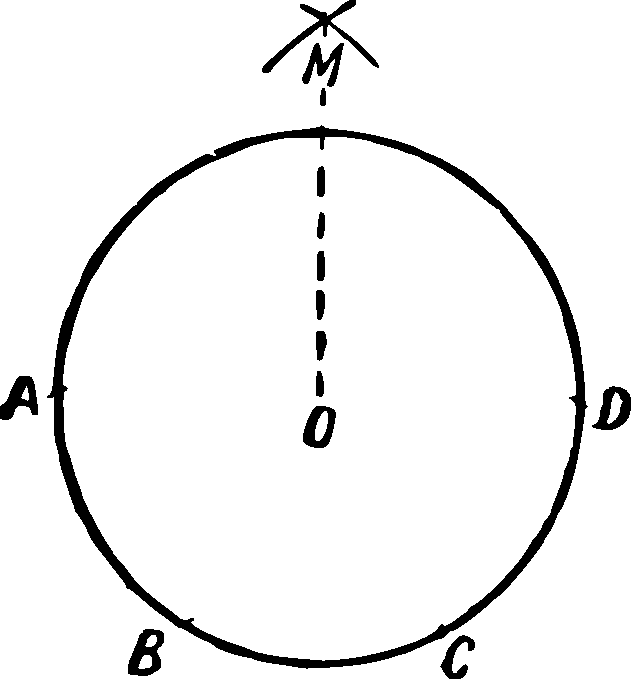
\includegraphics[width=\textwidth]{figures/ch-10/fig-145.pdf}
\sidecaption{Divide the circle into four equal parts using the ruler.\label{fig-145}}
\end{marginfigure}


\ans Suppose we need to divide circle $O$ (\figr{fig-145}) into four parts. From an arbitrary point $A$, we lay off three times the radius of the circle along the circumference: we obtain points $B$, $C$, and $D$. It is easy to see that the distance $AC$, the chord of the arc constituting 1/3 of the circle, is the side of the inscribed equilateral triangle and therefore equals \( r \sqrt{3} \), where \( r \) is the radius of the circle. $AD$ is obviously the diameter of the circle. From points $A$ and $D$, with a radius equal to $AC$, we draw arcs intersecting at point $M$. We will show that the distance $MO$ is equal to the side of the square inscribed in our circle. In triangle $AMO$, the leg $MO$ equals \( \sqrt{AM^{2} - AO^{2}} = \sqrt{3r^{2} - r^{2}} = r\sqrt{2} \), i.e., the side of the inscribed square. Now, using the compass set to MO, we lay off four points on the circle in succession to obtain the vertices of the inscribed square, which will obviously divide the circle into four equal parts.


\ques Here is another, easier problem of the same kind. Without a ruler, increase the distance between given points $A$ and $B$ (see \figr{fig-146}) by five times, or more generally, by any given factor.

\begin{marginfigure}%[h!]
\centering
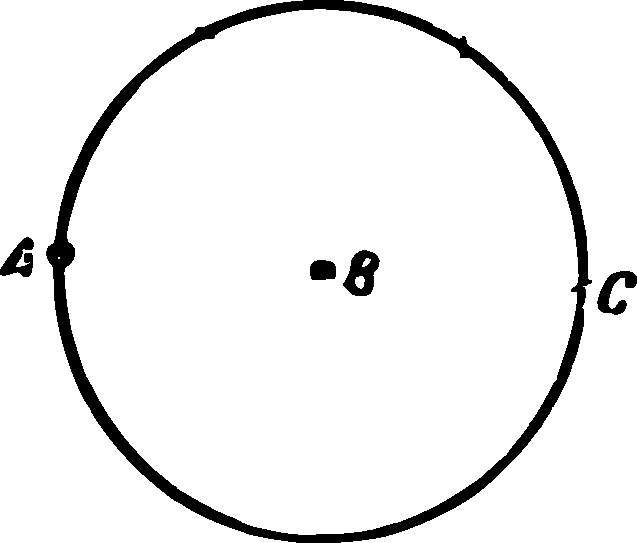
\includegraphics[width=\textwidth]{figures/ch-10/fig-146.pdf}
\sidecaption{How can we increase the distance between points $A$ and $B$ by a factor $n$ (an integer) using only a compass?\label{fig-146}}
\end{marginfigure}

\ans From point $B$, draw a circle with radius $AB$ (see \figr{fig-146}). Along this circle, measure the distance $AB$ three times from point $A$: you get point $C$, which is obviously diametrically opposite to $A$. The distance $AC$ is twice the distance $AB$. By drawing a circle from point $C$ with radius $BC$, we can similarly find a point diametrically opposite to $B$ and, therefore, three times the distance $AB$ from $A$, and so on.


\section{Simple Trisector}
\label{sec-10.4}

Using only a compass and an unmarked ruler, it is impossible to divide an arbitrarily given angle into three equal parts. However, mathematics does not completely rule out the possibility of performing this division using some other devices. Many mechanical devices have been invented to achieve this goal. These devices are called trisectors. You can easily make a simple trisector from stiff paper, cardboard, or thin metal. It will serve as an auxiliary drawing tool.


\begin{figure}[h!]
\centering
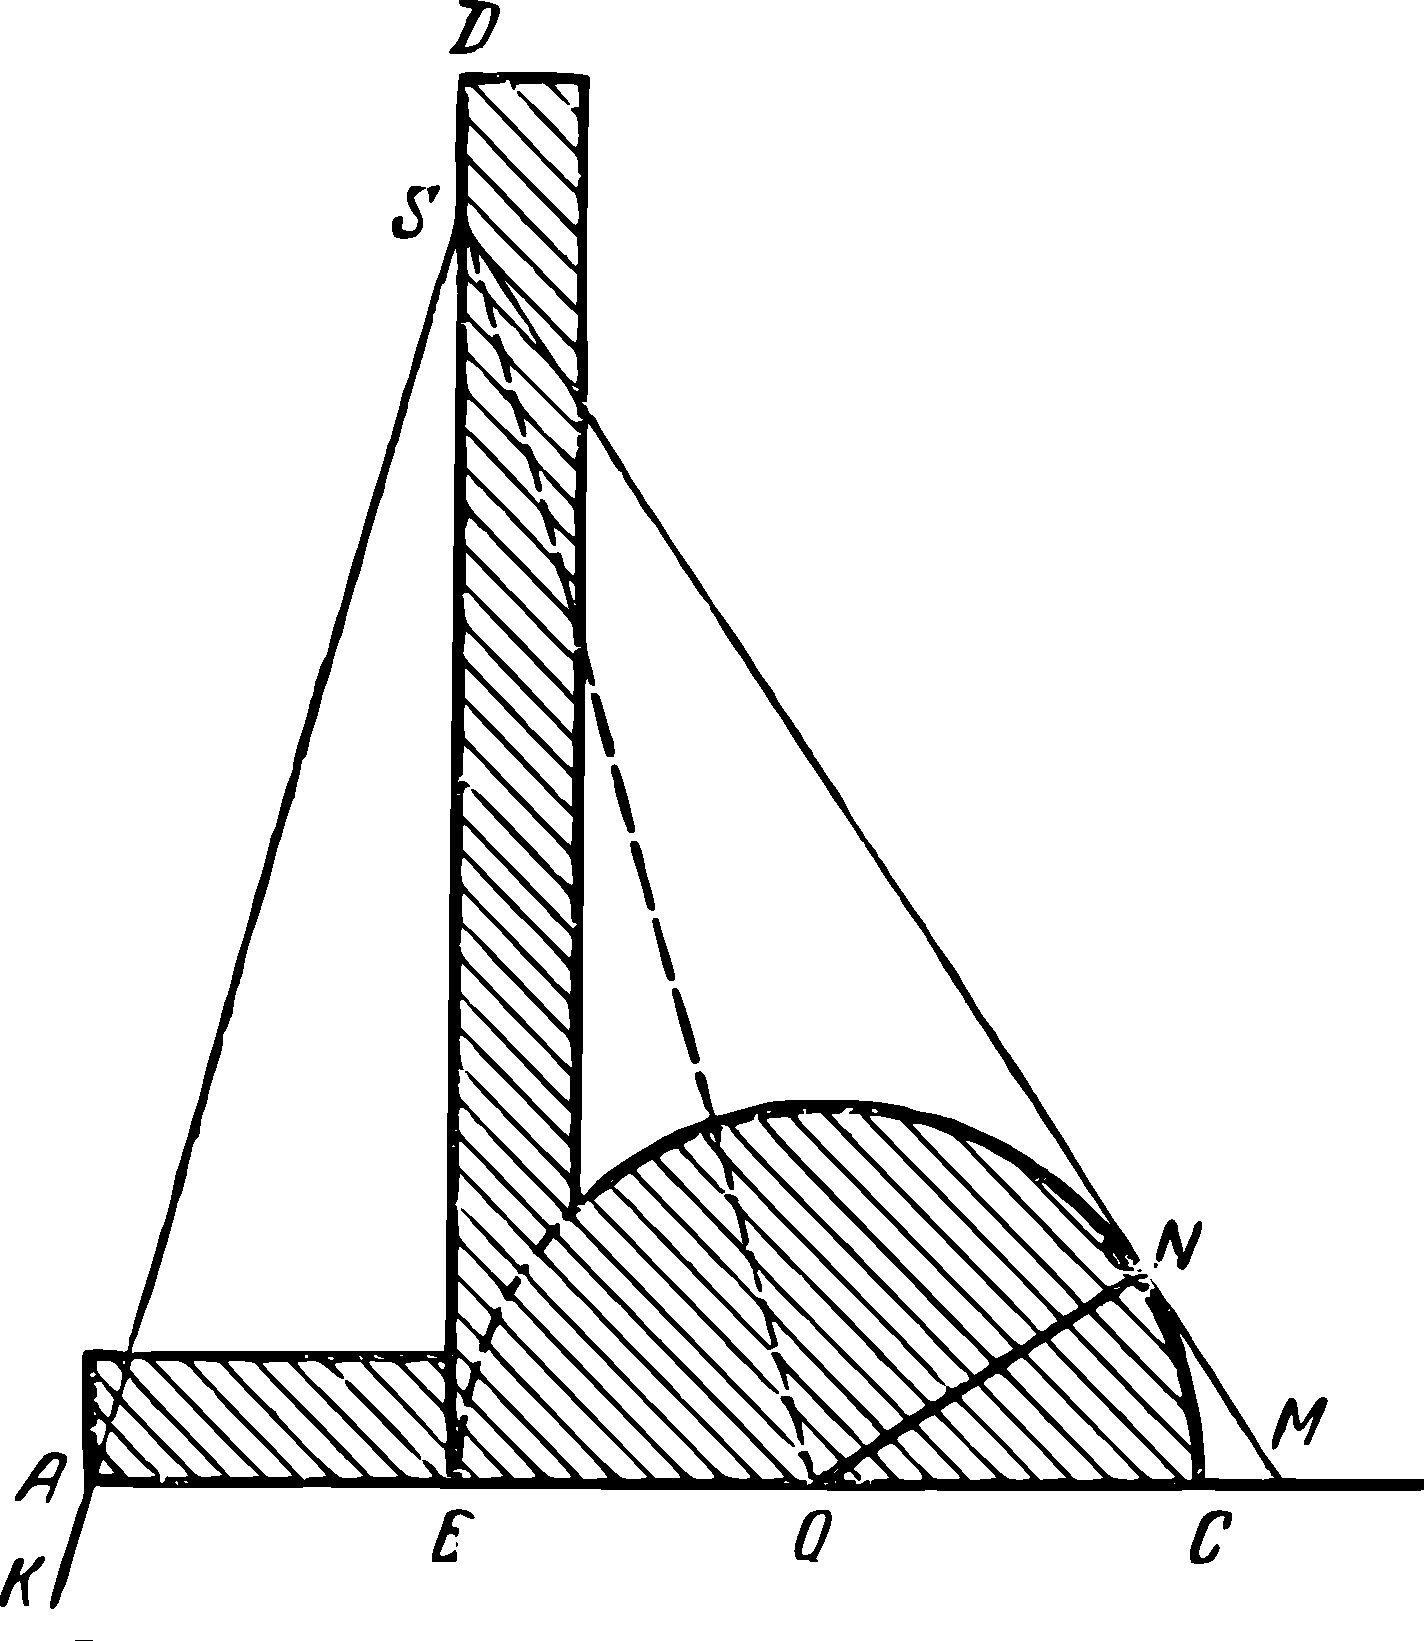
\includegraphics[width=0.8\textwidth]{figures/ch-10/fig-147.pdf}
\sidecaption[][-1cm]{Trisector and its usage scheme.\label{fig-147}}
\end{figure}


In \figr{fig-146}, the trisector is shown at full scale (shaded figure). The strip $AB$ adjacent to the semicircle is equal in length to the radius of the semicircle. The edge of the strip $BD$ forms a right angle with the line $AC$; it touches the semicircle at point $B$; the length of this strip is arbitrary. The same figure shows how to use the trisector. For example, let’s say you need to divide the angle $KSM$ (\figr{fig-146}) into three equal parts.

Place the trisector so that the vertex of the angle $S$ is on the line $BD$, one side of the angle passes through point $A$, and the other side touches the semicircle at point\sidenote[][-2.5cm]{The possibility of fitting our trisector into a given angle follows from a simple property of the points on the rays dividing the angle into three equal parts: if from any point $O$ on the ray $SO$ you draw segments $ON \perp SM$ and $OA \perp SB$ (\figr{fig-147}), then we have: $AB = OB = ON$. The reader can easily prove this for themselves.}. Then draw straight lines $SB$ and $SO$, and the division of the given angle into three equal parts is complete. To prove this, connect the centre of the semicircle $O$ to the point of tangency $N$ with a straight line segment. It is easy to see that triangle $ASB$ is equal to triangle $SBO$, and triangle $SBO$ is equal to triangle $OSN$. From the equality of these three triangles, it follows that angles $ASB$, $BSO$, and $OSN$ are equal to each other, which is what was required to be proved.

This method of angle trisection is not purely geometric; it can be called mechanical.


\section{Clock Trisector}
\label{sec-10.5}

\ques Is it possible to divide a given angle into three equal parts using a compass, a ruler, and a clock?

\ans Yes, it is possible. Transfer the figure of the given angle onto transparent paper and, at the moment when both clock hands overlap, place the drawing onto the clock face so that the vertex of the angle coincides with the centre of the clock hands' rotation and one side of the angle aligns with the hands (\figr{fig-148}).

\begin{figure}[h!]
\centering
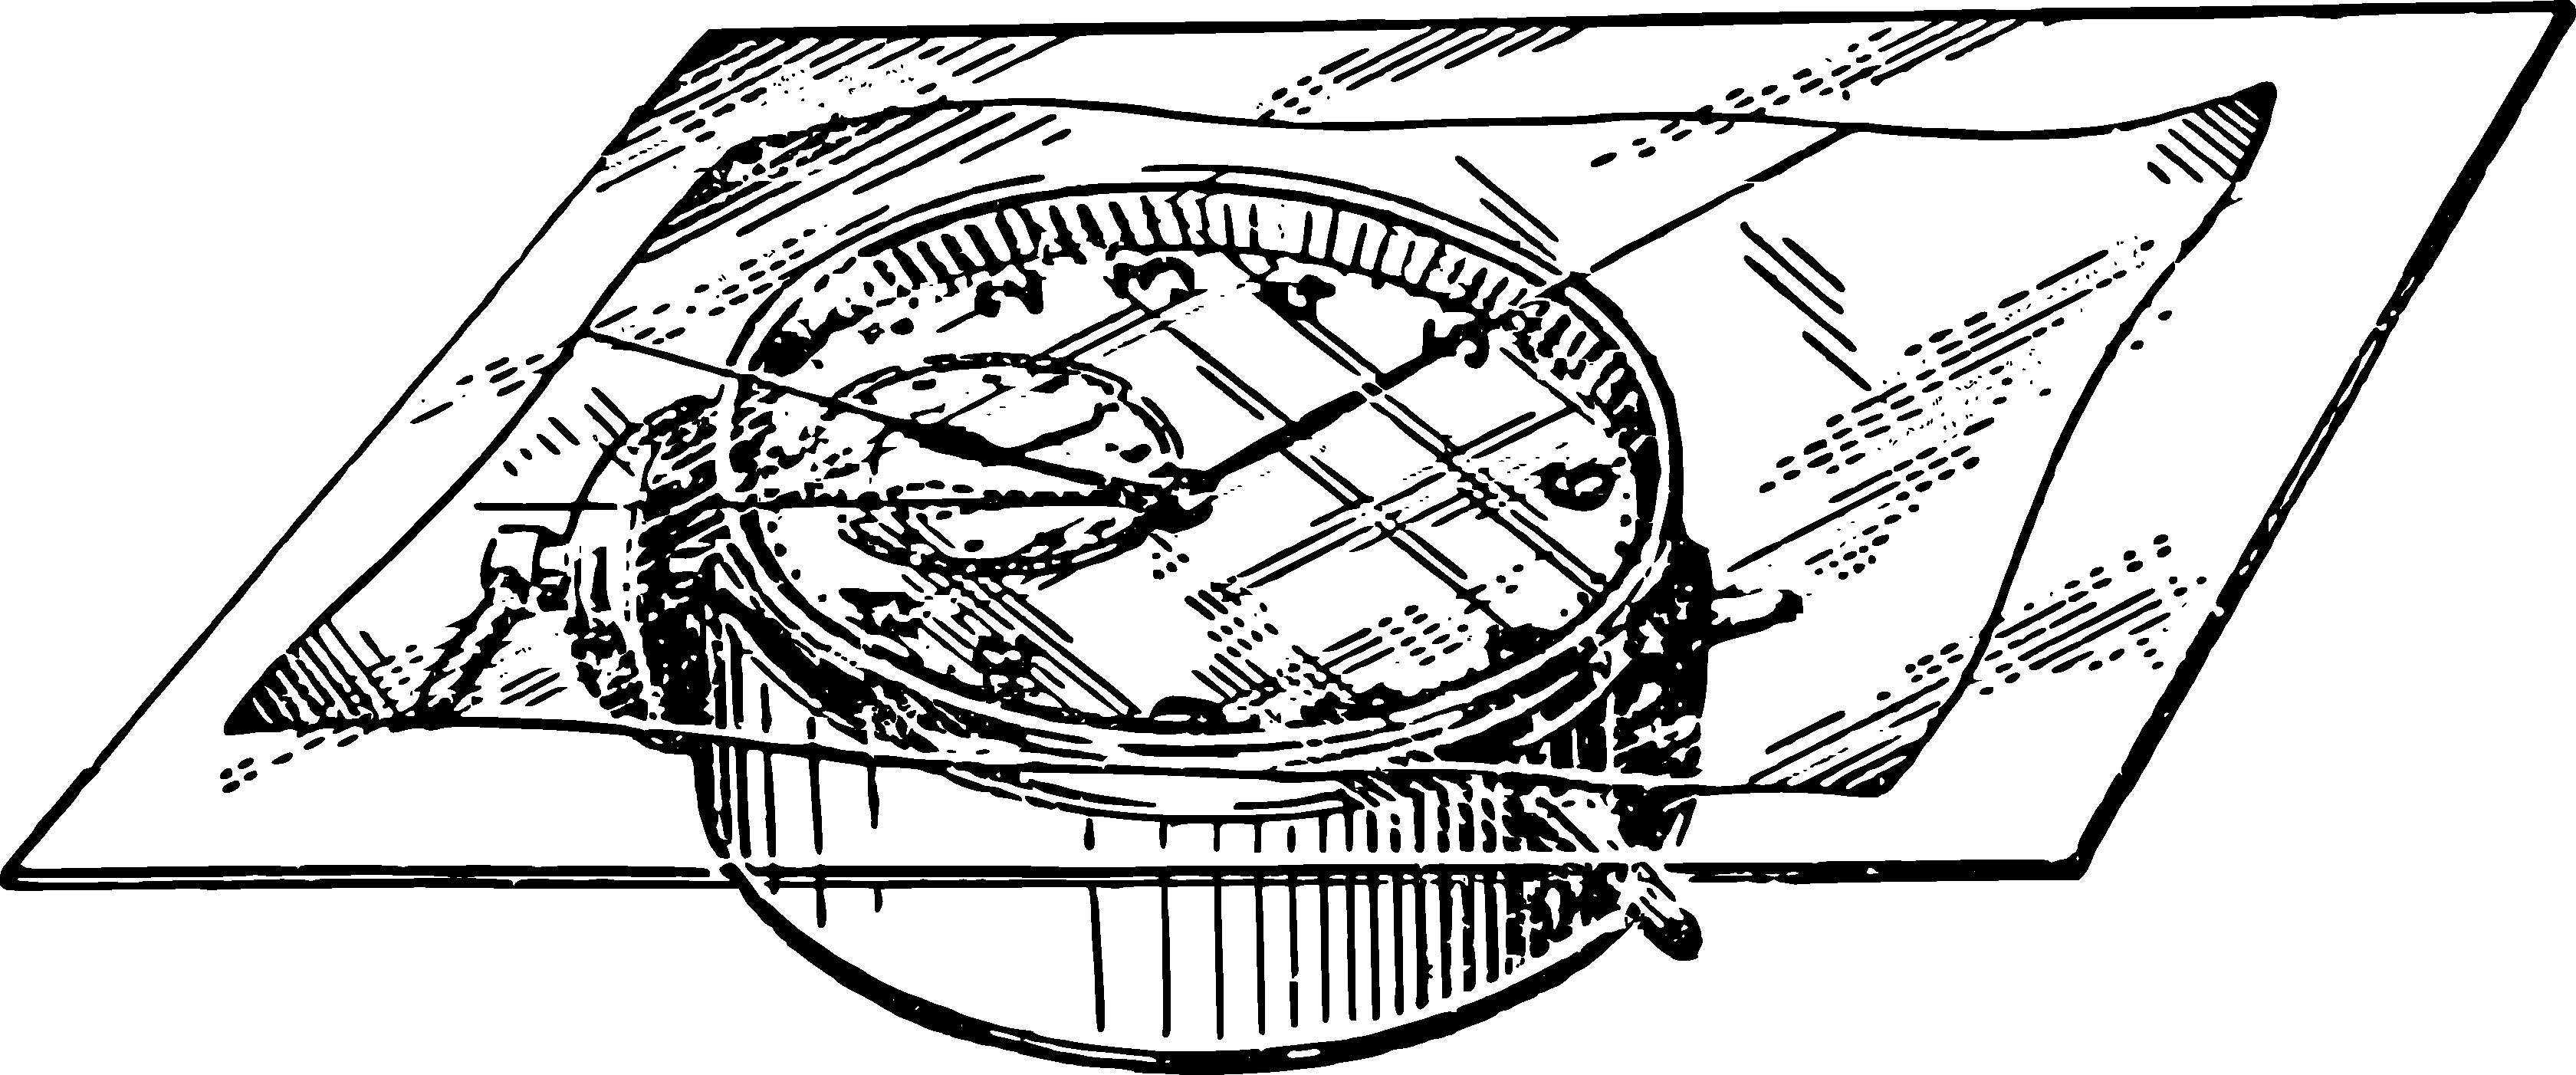
\includegraphics[width=0.85\textwidth]{figures/ch-10/fig-148.pdf}
\sidecaption{Clock Trisector.\label{fig-148}}
\end{figure}


At the moment when the minute hand moves to coincide with the direction of the second side of the given angle (or move it manually), draw a ray from the vertex of the angle in the direction of the hour hand. This creates an angle equal to the angle of the hour hand’s movement. Now, using a compass and a ruler, double this angle and then double the doubled angle again (the method for doubling an angle is well known in geometry). The angle obtained in this way will be one-third of the given angle.

Indeed, every time the minute hand describes a certain angle \( \alpha \), the hour hand moves by an angle that is 12 times smaller: \( \alpha/12 \), and after quadrupling this angle, you get \( \alpha/12 \times 4 = \alpha/3 \).



\section{Dividing a Circle}
\label{sec-10.6}

Radio enthusiasts, designers, builders of various models, and enthusiasts sometimes face the practical problem of cutting a given sheet into a regular polygon with a specified number of sides.

This task can be reduced to:

Dividing a circle into \( n \) equal parts, where \( n \) is an integer.



Let's put aside the obvious solution using a protractor—since that's essentially an ``eyeball'' method—and consider a geometric solution using a compass and a ruler.

First, let's address the question: into how many equal parts can a circle theoretically be divided using a compass and a ruler? Mathematicians have fully resolved this: not into any number of parts.\sidenote{For details, see the geometry textbook.}

Possible divisions: 
\begin{equation*}%
2,\,\, 3, \,\, 4, \,\, 5, \,\, 6, \,\, 8, \,\, 10,  \,\, 12, \,\, 15, \,\, 16, \,\, 17, \,\,  257, \,\, \text{etc.}
\end{equation*}
Impossible divisions: 
\begin{equation*}%
7,\,\, 9, \,\, 11, \,\, 13, \,\, 14, \,\, \text{etc.}
\end{equation*}
Furthermore, there is no single method for constructing these divisions; the technique for dividing into 15 parts is different from that for 12 parts, and so on, making it difficult to remember all methods.

A practical geometric method is needed -- one that is approximate but simple and general enough for dividing a circle into any number of equal arcs.

Unfortunately, geometry textbooks do not yet address this issue, so here we will present an interesting method for an approximate geometric solution to this problem.


\begin{marginfigure}%[h!]
\centering
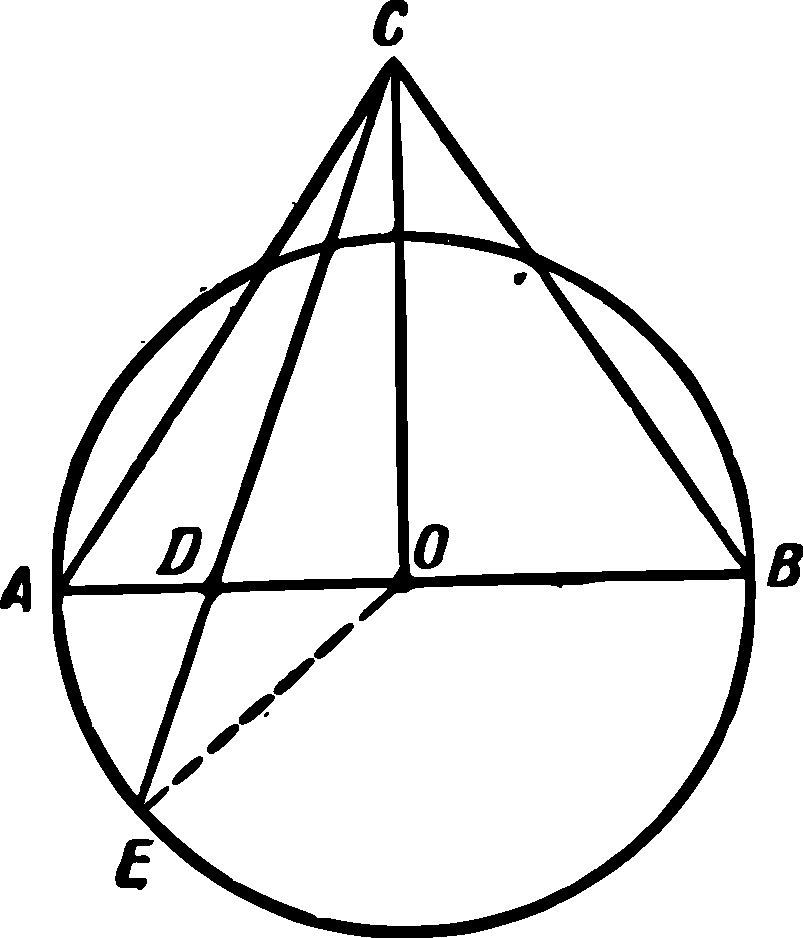
\includegraphics[width=\textwidth]{figures/ch-10/fig-149.pdf}
\sidecaption{An approximate geometric method of dividing a circle into $n$ equal parts.\label{fig-149}}
\end{marginfigure}



For example, let's say we need to divide a given circle (\figr{fig-149}) into nine equal parts. Construct a scalene triangle $ACB$ on some diameter $AB$ of the circle and divide the diameter $AB$ at point $D$ in the ratio $AD:AB = 2:9$ (generally $AD:AB = 2:n$).

Connect points $C$ and $D$ with a line segment and extend it to intersect the circle at point $E$. Then, the arc $\wideparen{AE}$ will be approximately 1/9 of the circle (generally $\wideparen{AE} = \ang{360}/n$), or chord $AE$ will be the side of a regular inscribed nonagon ($n$-gon).

The relative error in this method is about 0.8\%.


If we express the relationship between the central angle AOE, formed in the described construction, and the number of divisions \( n \), we get the following exact formula:
\begin{equation*}%
\tan \wideparen{AOE} = \frac{\sqrt{3}}{2} \cdot \frac{n^2 + 16n - 32 - n}{n - 4}
\end{equation*}
For larger values of \( n \), this can be approximated by the formula:
\begin{equation*}%
\tan \wideparen{AOE} = 4 \, \sqrt{3} \cdot \left(\frac{1}{n} - \frac{2}{n^2}\right)
\end{equation*}
On the other hand, for exact division of the circle into \( n \) equal parts, the central angle should be equal to \(\ang{360}/n \). By comparing the angle  \(\ang{360}/n \) with the angle $AOE$, we obtain the error made when considering the arc AE as \( 1/n \) part of the circle. The following table shows the error for some values of \( n \).

\begin{table*}
\centering
\begin{small}
\begin{tabular}{p{1cm}lllllllll}
\toprule
$n$	& 3	& 4	& 5	& 6	& 7	& 8	& 10	 & 20 & 60 \\
\midrule
$\ang{360}/n$ &	\ang{120} & 	\ang{90} & 	\ang{72} & 	\ang{60} & 	\ang{51;26}	& \ang{45} & \ang{36} & \ang{18} & \ang{6}\\
$\wideparen{AOE}$	&	\ang{120} & 	\ang{90} & 	\ang{71;57} & 	\ang{60} & 	\ang{51;31}	& \ang{45;11} & \ang{36;21} & \ang{18;38} & \ang{6;26}\\
Error \% & 0 & 0 & 0.07 & 0 & 0.17 & 0.41 & 0.97 &  3.5 & 7.2 \\
\bottomrule
\end{tabular}
\end{small}
\end{table*}

As can be seen from the table, this method can approximately divide the circle into 5, 7, 8, or 10 parts with a small relative error ranging from 0.07\% to 1\%, which is quite acceptable for most practical purposes. However, as the number of divisions \( n \) increases, the accuracy of the method decreases noticeably, i.e., the relative error increases, but studies show that for any \( n \), the error does not exceed 10\%.




\section[Billiard Ball Problem]{Direction of the Shot (Billiard Ball Problem)}
\label{sec-10.7}

Hitting a billiard ball into a pocket by making it bounce off one, two, or even three rails of the table means, first of all, solving a geometric ``construction'' problem in your mind.

It's crucial to accurately ``eyeball'' the first point of impact on the rail; the subsequent path of the elastic ball on a good table will be determined by the law of reflection (\emph{the angle of incidence equals the angle of reflection}).



\begin{figure}[h!]
\centering
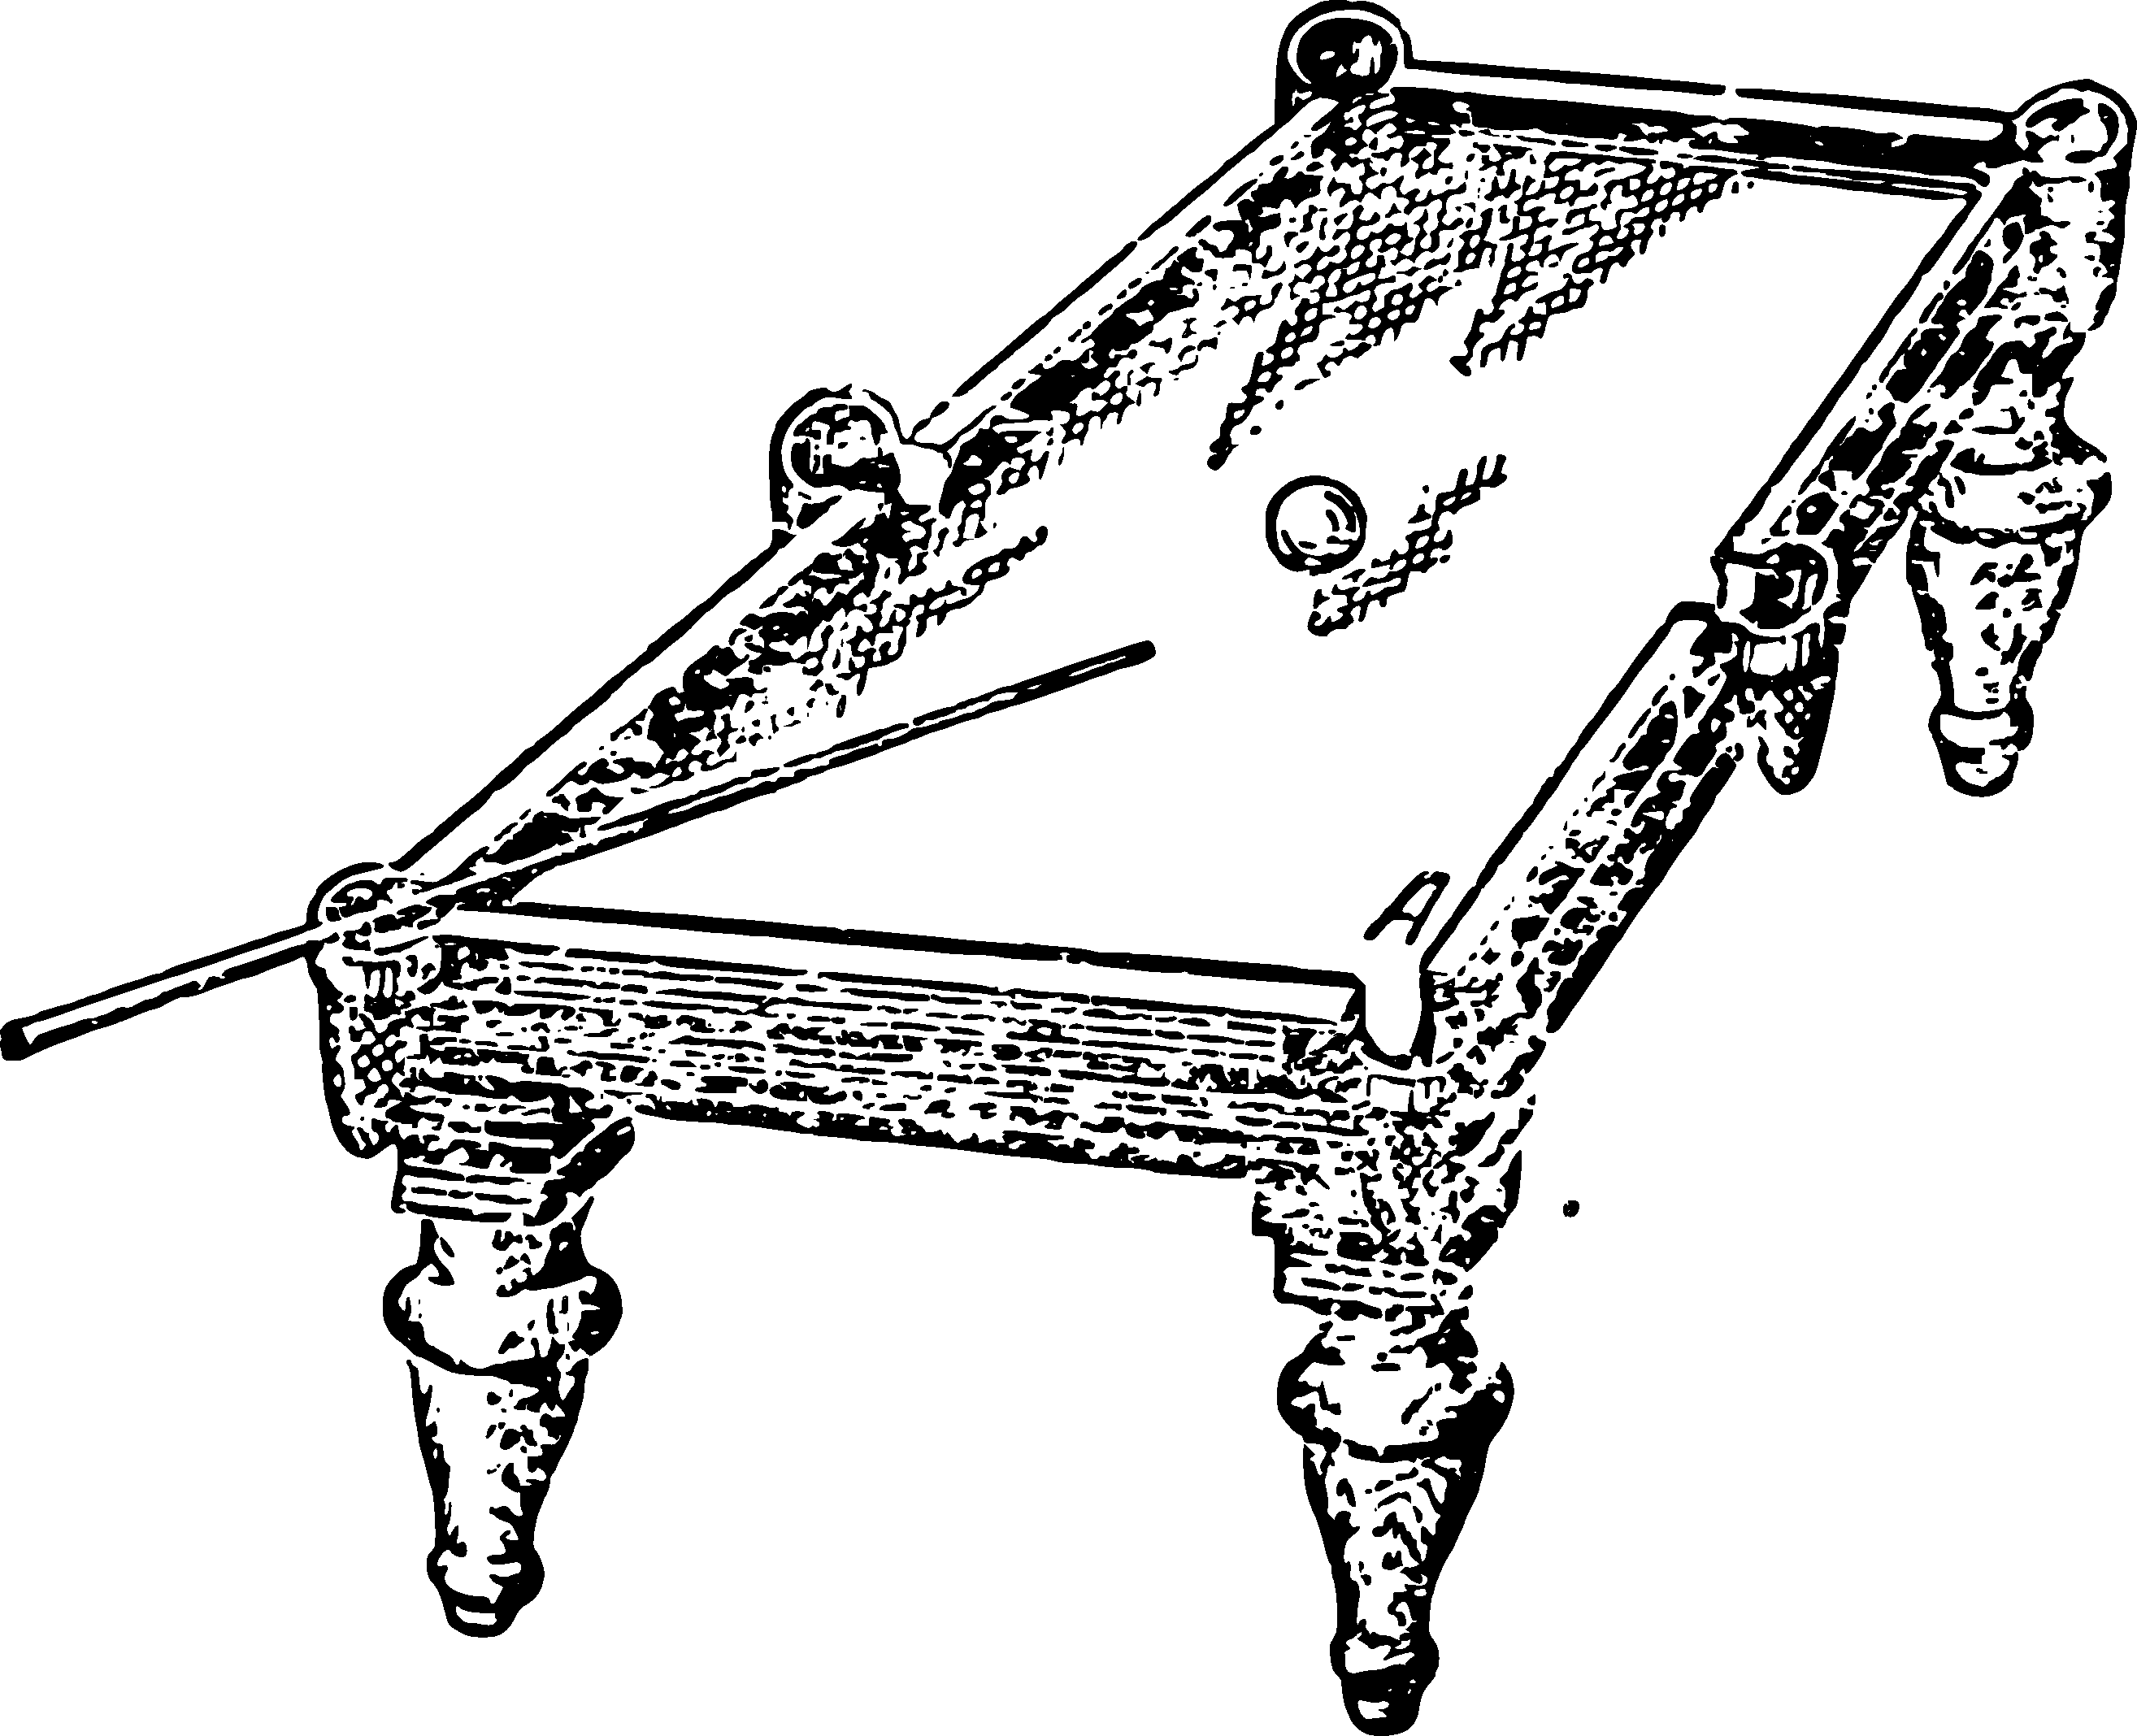
\includegraphics[width=0.7\textwidth]{figures/ch-10/fig-150.pdf}
\sidecaption{A geometric problem on a billiard table.\label{fig-150}}
\end{figure}




\ques What geometric concepts can help you find the direction of the shot so that a ball located, for example, in the middle of the billiard table, after three bounces, lands in pocket $A$? (\figr{fig-150}).


\ans You need to imagine that three more tables are placed along the short side of the billiard table, and aim in the direction of the farthest pocket on the third imaginary table.

\figr{fig-151} helps clarify this statement. Let \( OabcA \) be the path of the ball. If you flip the ``table'' $ABCD$ around $CD$ by \ang{180} degrees, it will occupy position $I$, then flip it again around $AD$ and once more around $BC$, it will occupy position $III$. As a result, pocket $A$ will be at the point marked $A_{1}$.

Based on the obvious equality of the triangles, you can easily prove that \( ab_{1} = ab \), \( b_{1}c_{1} = bc \), and \( c_{1}A_{1} = cA \), i.e., the length of the straight line \( OA_{1} \) is equal to the length of the broken line \( OabcA \).


\begin{marginfigure}%[h!]
\centering
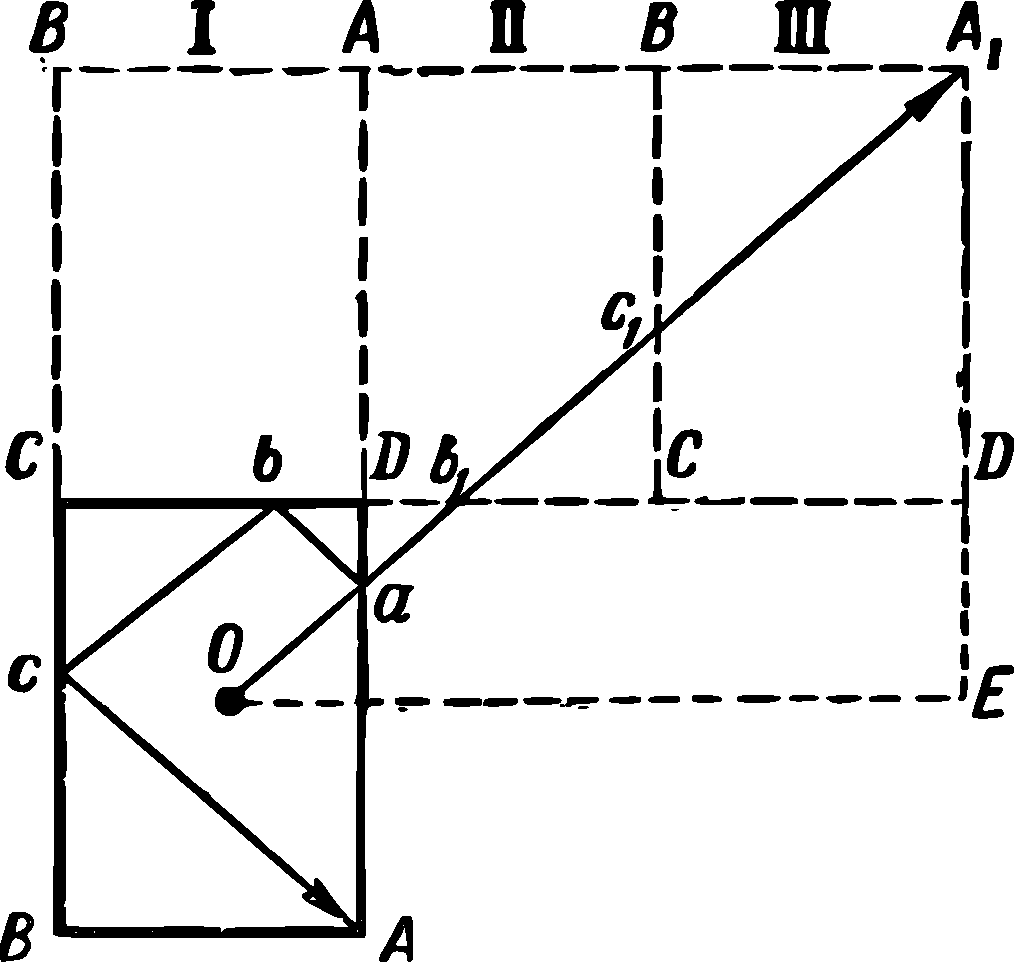
\includegraphics[width=\textwidth]{figures/ch-10/fig-151.pdf}
\sidecaption{A geometric problem on a billiard table.\label{fig-151}}
\end{marginfigure}


Therefore, aiming at the imaginary point $A_{1}$ will cause the ball to travel along the path \( OabcA \), and it will land in pocket $A$.

Let’s consider another question: under what condition will the sides \( OE \) and \( A_{1}E \) of the right triangle \( A_{1}EO \) be equal?

It is easy to establish that \( OE = 5/2 \, AB \) and \( A_{1}E = 3/2\, BC \). If \( OE = A_{1}E \), then \( 5/2 AB = 3/2\, BC \), or \( AB = 3/5 \, BC \).

Thus, if the short side of the billiard table is 3/5 of the long side, then \( OE = EA_{1} \); in this case, you can direct the shot of a ball located in the middle of the table at a \ang{45} angle to the rail.

\section{The ``Smart'' Ball}
\label{sec-10.8}

Simple geometric constructions just helped us solve a problem involving a billiard ball. Now let's have the same billiard ball solve an interesting, old problem on its own.

Is that even possible? -- A ball can't think. True, but when a calculation needs to be performed, and we know the operations and their order, such a calculation can be entrusted to a machine, which will perform it quickly and without error.

Many mechanisms have been invented for this purpose, from simple mechanical calculators to complex electronic machines.

In leisure time, people often entertain themselves with the problem of how to pour a specific amount of water from a filled container of known capacity using two other empty containers, also of known capacities.

Here is one of many problems of this kind:

Divide the contents of a 12-bucket barrel in half using two empty barrels of nine buckets and five buckets.

To solve this problem, you don’t need to experiment with actual barrels. All necessary ``pourings'' can be done on paper with a simple scheme:

%\begin{table*}

\begin{small}
\begin{center}
\begin{tabular}{@{}r *{9}{c}@{}}
\toprule
9 Buckets & 0 & 7\tikzmark{a3} & 7\tikzmark{a6} & 2 & 2\tikzmark{a9} & 0 & 9\tikzmark{a11} & 6 & 6 \\
5 Buckets & 5\tikzmark{a2} & 5\tikzmark{a4} & 0 & 5\tikzmark{a7} & 0 & 2\tikzmark{a10} & 2 & 5\tikzmark{a12} & 0 \\
12 Buckets\tikzmark{a1} & 7 & 0 & 5\tikzmark{a5} & 5 & 
   \makebox[\widthof{0}][c]{10}\tikzmark{a8} & 
   \makebox[\widthof{0}][c]{10} & 
   1 & 1 & 6\tikzmark{a13} \\ 
\bottomrule
\end{tabular}
\end{center}
\end{small}
%\end{table*}
\begin{tikzpicture}[overlay, remember picture, 
  shorten >=8pt, 
  shorten <=3pt, 
  transform canvas={yshift=.33\baselineskip}]
    \draw [-stealth, red, thick] ({pic cs:a1}) -- ({pic cs:a2});
    \draw [-stealth, red, thick] ({pic cs:a2}) -- ({pic cs:a3});
    \draw [-stealth, red, thick] ({pic cs:a4}) -- ({pic cs:a5});
    \draw [-stealth, red, thick] ({pic cs:a6}) -- ({pic cs:a7});
    \draw [-stealth, red, thick] ({pic cs:a7}) -- ({pic cs:a8});
    \draw [-stealth, red, thick] ({pic cs:a9}) -- ({pic cs:a10});
    \draw [-stealth, red, thick] ({pic cs:a10}) -- ({pic cs:a11});
    \draw [-stealth, red, thick] ({pic cs:a11}) -- ({pic cs:a12});
    \draw [-stealth, red, thick] ({pic cs:a12}) -- ({pic cs:a13}); 
\end{tikzpicture}

% https://tex.stackexchange.com/questions/718439/aligning-arrows-in-table

In each column, record the result of the current pouring. 

Fill the five-bucket barrel. The nine-bucket barrel is empty (0), and seven buckets remain in the 12-bucket barrel. 

Pour the seven buckets from the 12-bucket barrel into the nine-bucket barrel, and so on.

The scheme has nine columns, indicating that nine pourings were needed to solve the problem.

Try to find your own solution to the proposed problem, establishing a different order of pourings.

After several attempts, you will undoubtedly succeed, as the proposed pouring scheme is not the only possible one; however, with a different order of pourings, you might need more than nine.

In this context, it is interesting to explore the following:
\begin{enumerate}
\item Can a specific order of pourings be established that can be followed in all cases, regardless of the capacities of the containers?
\item Can any possible amount of water be poured from a third container using two empty containers, e.g., for example, from a 12-bucket barrel using barrels in 9 and 5 buckets, one bucket of water, or two buckets, or three, four, etc. to 11?
\end{enumerate}

The ``smart'' ball will answer all these questions if we now construct a special ``billiard table'' for it.

Draw a sheet of paper in a slant grid so that the cells are equal rhombuses with acute angles of \ang{60}, and construct the figure $OABCD$ as shown in \figr{fig-152}.



\begin{figure}[h!]
\centering
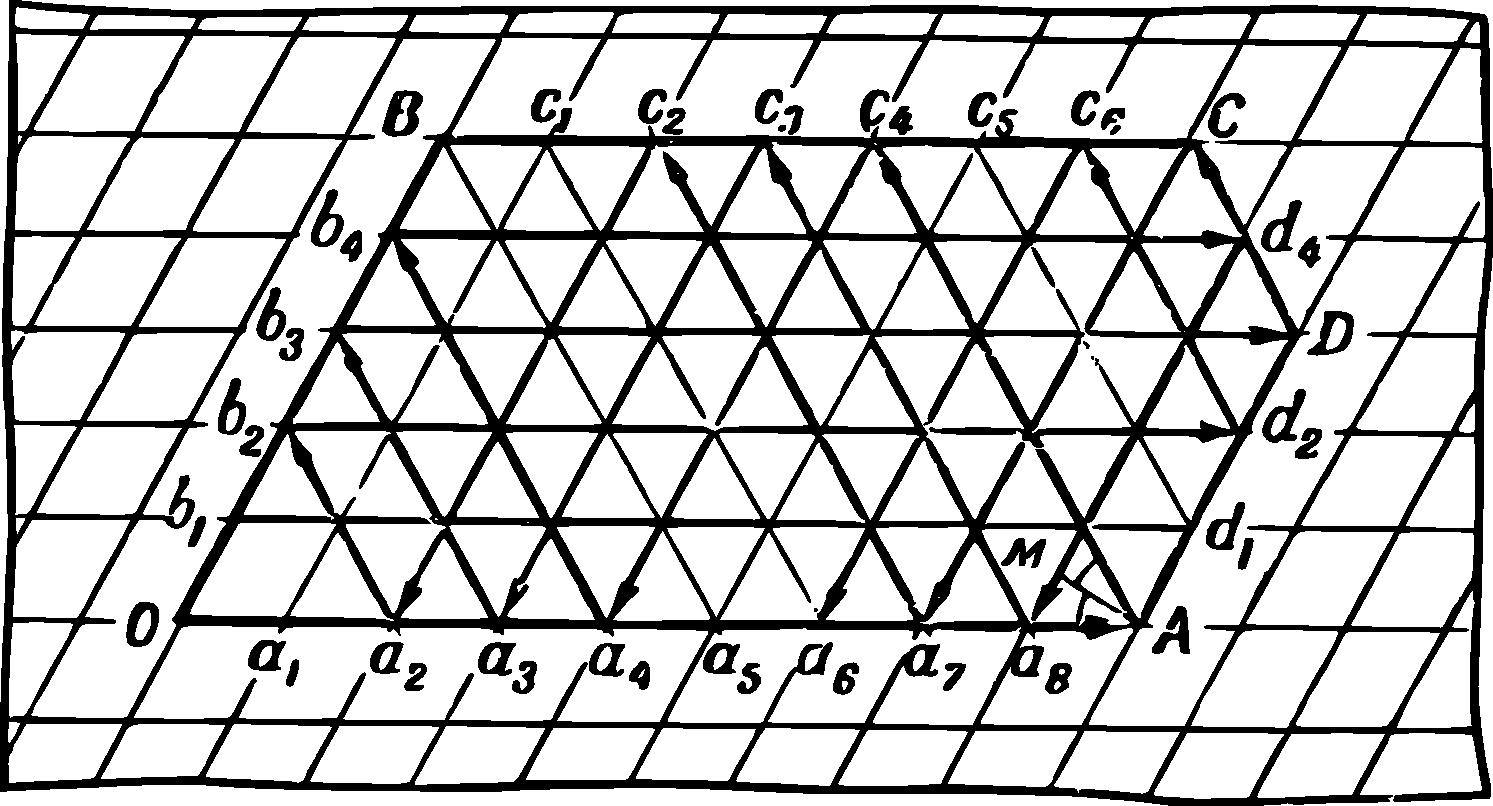
\includegraphics[width=0.9\textwidth]{figures/ch-10/fig-152.pdf}
\sidecaption{The ``mechanism'' of the ``smart'' ball.\label{fig-152}}
\end{figure}


This will be the ``billiard table''. If you push the billiard ball along $OA$, it will bounce off the rail $AD$ exactly according to the law \emph{the angle of incidence equals the angle of reflection} $(\angle OAM = \angle MAc_{4})$, and the ball will roll along the straight line $Ac_{4}$ connecting the vertices of the small rhombuses; it will bounce at point $c_{4}$ from the edge BC and roll along the line $c_{4}a_{4}$, then along the lines $a_{4}b_{4}$, $b_{4}d_{4}$, $d_{4}a_{8}$, and so on.

According to the conditions of the task, we have three barrels: nine, five And 12 buckets. In accordance with this, we will construct the figure so that the side $OA$ contains nine cells, $OB$ contains five cells, $AD$ contains three cells $(12 - 9 = 3)$, $BC$ contains seven cells\sidenote{A filled barrel is always the largest of the three. Let the capacity of empty barrels $a$ and $b$ be filled with $c$. If $c \geqslant a + b$, then the ``billiard table'' should be built in the form of a parallelogram with the sides $a$ and $b$ of the cells.} $(12 - 5 = 7)$.


Note that each point on the sides of the figure is separated by a certain number of cells from the sides $OB$ and $OA$. For example, from point $c_{4}$ -- it is four cells to $OB$ and five cells to $OA$, from point $a_{4}$ -- it is four cells to OB and zero cells to $OA$ (because it lies on $OA$), from point $d_{4}$ --, it is eight cells to $OB$ and four cells to $OA$, and so on.

Thus, each point on the sides of the figure where the billiard ball hits determines two numbers.

Let us agree that the first number, i.e., the number of cells separating the point from $OB$, indicates the number of buckets of water in the nine-bucket barrel, and the second number, i.e., the number of cells separating the same point from $OA$, indicates the number of buckets of water in the five-bucket barrel. The remaining amount of water will obviously be in the 12-bucket barrel.

Now everything is prepared to solve the problem using the billiard ball.

Send it again along $OA$ and, decoding each point where it hits the edge as indicated, follow its movement at least to point $a_{6}$ (\figr{fig-152}).

The first point of impact is $A \,(9; 0)$; this means the first transfer should result in the following distribution of water:

\begin{small}
\begin{center}
\begin{tabular}{@{}r *{1}{c}@{}}
\toprule
9 Buckets & 9  \\
5 Buckets & 0 \\
12 Buckets & 3\\ 
\bottomrule
\end{tabular}
\end{center}
\end{small}

This is feasible. The second point of impact is $c_{4}\, (4; 5)$; therefore, the ball recommends the following result for the second transfer:

\begin{small}
\begin{center}
\begin{tabular}{@{}r *{3}{c}@{}}
\toprule
9 Buckets & 9  & 4 &\\
5 Buckets & 0 & 5 & \\
12 Buckets & 3 & 3 & \\ 
\bottomrule
\end{tabular}
\end{center}
\end{small}

This is also feasible. The third point of impact is $a_{4}\, (4; 0)$; for the third transfer, the ball suggests returning five buckets to the 12-bucket barrel:

\begin{small}
\begin{center}
\begin{tabular}{@{}r *{4}{c}@{}}
\toprule
9 Buckets & 9  & 4 & 4 & \\
5 Buckets & 0 & 5 & 0 & \\
12 Buckets & 3 & 3 & 8 &\\ 
\bottomrule
\end{tabular}
\end{center}
\end{small}

The fourth point of impact is $b_{4}\, (0; 4)$; the result of the fourth transfer:

\begin{small}
\begin{center}
\begin{tabular}{@{}r *{5}{c}@{}}
\toprule
9 Buckets & 9  & 4 & 4 & 0 & \\
5 Buckets & 0 & 5 & 0 & 4 & \\
12 Buckets & 3 & 3 & 8 & 8 & \\ 
\bottomrule
\end{tabular}
\end{center}
\end{small}

The fifth point of impact is $d_{4}\, (8; 4)$, and the ball insists on transferring eight buckets to the empty nine-bucket barrel:

\begin{small}
\begin{center}
\begin{tabular}{@{}r *{6}{c}@{}}
\toprule
9 Buckets & 9  & 4 & 4 & 0 & 8 & \\
5 Buckets & 0 & 5 & 0 & 4 & 4 & \\
12 Buckets & 3 & 3 & 8 & 8 & 0 &\\ 
\bottomrule
\end{tabular}
\end{center}
\end{small}


Continue to follow the ball, and you will get the following table:

\begin{table*}
\centering
\begin{small}
\begin{tabular}{@{}r *{18}{c}@{}}
\toprule
9 Buckets & 9  & 4 & 4 & 0 & 8 & 8 & 3 & 3 & 0& 9 & 7 & 7 & 2 & 2 & 0 & 9 & 6 & 6\\
5 Buckets & 0 & 5 & 0 & 4 & 4 & 0 & 5 & 0 & 3 & 3 & 5 & 0 & 5 & 0 & 2 & 2 & 5 & 0\\
12 Buckets & 3 & 3 & 8 & 8 & 0 & 4 & 4 & 9 & 9 & 0 & 0  & 5 & 5 & 10 & 10 & 1  & 1 & 6\\ 
\bottomrule
\end{tabular}
\end{small}
\end{table*}

So, after a series of transfers, the goal is achieved: six buckets of water in each of the two barrels. The ball has solved the problem!


However, the ball turned out not to be very smart.

It solved the problem in 18 moves, while we managed to solve it in nine moves (see the first table).

However, the ball can also shorten the series of transfers. Push it first along $OB$, stop it at point $B$, then push it again along $BC$, and then let it move as agreed -- according to the law of \emph{the angle of incidence equals the angle of reflection}. This will result in a shorter series of transfers.

If you allow the ball to continue moving after point $a_{6}$, you can easily verify that in the case under consideration, it will cover all marked points on the sides of the figure (and generally all vertices of the rhombuses) and only after that will return to the starting point $O$. This means that from the 12-bucket barrel, you can pour any integer number of buckets from one to nine into the nine-bucket barrel, and from one to five into the five-bucket barrel.

But a task of this kind may not have the required solution.

How does the ball detect this?

Very simply: in this case, it will return to the starting point $O$ without hitting the desired point.


\figr{fig-153} shows the mechanism for solving the problem for barrels of nine, seven, and twelve buckets:

%\begin{table*}

%\begin{margintable}
%\centering
%\begin{sideways}
\begin{small}
\centering
\begin{center}
\begin{tabular}{@{}r *{12}{c}@{}}
\toprule
9 Buckets & 9  & 2 & 2 & 0 & 9 & 4 & 4 & 0 & 8 & 8 & 1 & 1 \\
7 Buckets & 0 & 7 & 0 & 2 & 2 & 7 & 0 & 4 & 4 & 0 & 7 & 0 \\
12 Buckets & 3 & 3 & 10 & 10 & 1 & 1 & 8  & 8 & 0 & 4 & 4  & 11 \\
\midrule
contd.\\
9 Buckets & 0 & 9 & 3 & 3 & 0 & 9 & 5 & 5 & 0 & 7 & 7 & 0 \\
7 Buckets & 1 & 1 & 7 & 0 & 3 & 3 & 7 & 0 & 5 & 5 & 0 & 7\\
12 Buckets & 11 & 2 & 2 & 9 & 9 & 0 & 0  & 7 & 7 & 0 & 5 & 5\\ 
\bottomrule
\end{tabular}
\end{center}
\end{small}
%\end{sideways}
%\end{margintable}
%\end{table*}


The ``mechanism'' shows that from a filled twelve-bucket barrel, using empty nine- and seven-bucket barrels, you can pour any number of buckets except half of its contents, i.e., except six buckets.


\begin{figure}[h!]
\centering
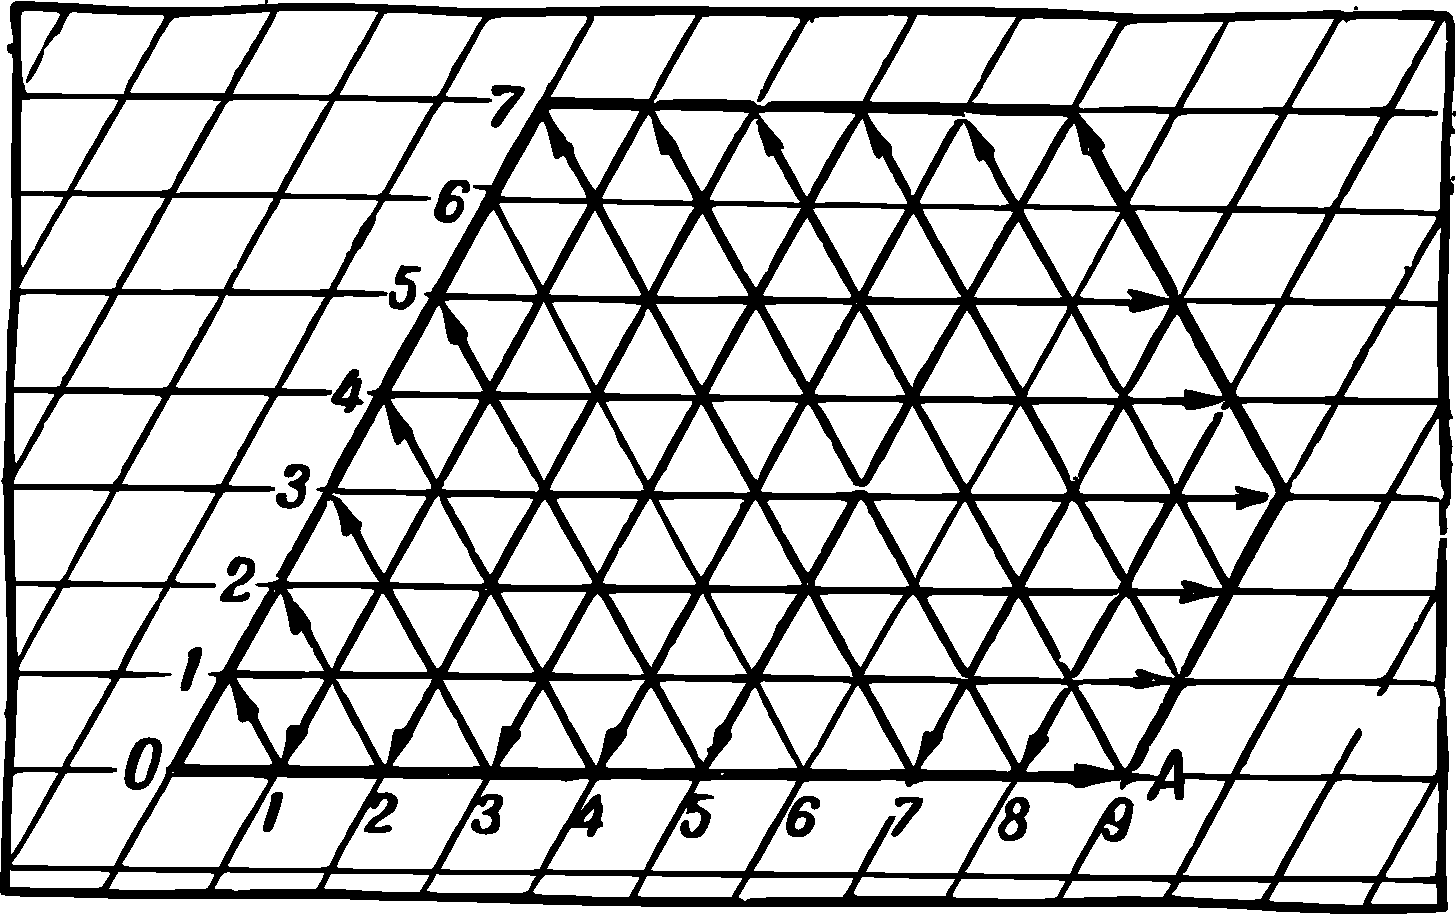
\includegraphics[width=0.9\textwidth]{figures/ch-10/fig-153.pdf}
\sidecaption{The ``mechanism'' shows that a full barrel of 12 buckets cannot be poured in half using empty barrels of nine and seven buckets.\label{fig-153}}
\end{figure}

\begin{small}
\begin{center}
\begin{tabular}{@{}r *{4}{c}@{}}
\toprule
6 Buckets & 6  & 3 & 3 & 0 \\
3 Buckets & 0 & 3 & 0 & 3  \\
8 Buckets & 2 & 2 & 5 & 5  \\ 
\bottomrule
\end{tabular}
\end{center}
\end{small}


\figr{fig-154} shows the mechanism for solving the problem for barrels of three, six, and eight buckets. Here, the ball makes four bounces and returns to the starting point $O$.


\begin{figure}[h!]
\centering
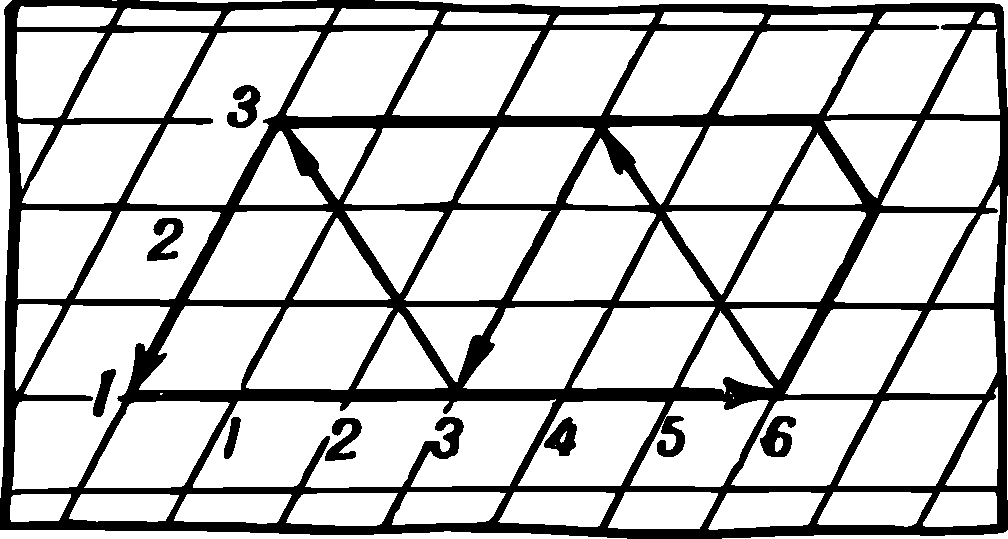
\includegraphics[width=0.7\textwidth]{figures/ch-10/fig-154.pdf}
\sidecaption{The ``mechanism'' for solving another transfer problem.\label{fig-154}}
\end{figure}


The corresponding table shows that in this case, it is impossible to pour four buckets or one bucket from the eight-bucket barrel.

Thus, our ``billiards'' with the ``smart'' ball indeed serves as an interesting and peculiar calculating machine, quite adept at solving pouring problems.


\section{In One Stroke}
\label{sec-10.9}



\ques Redraw on a sheet of paper the five figures shown in \figr{fig-155} and try to trace each of them in one stroke, i.e., without lifting your pencil from the paper and without tracing the same line more than once.



\begin{figure}[h!]
\centering
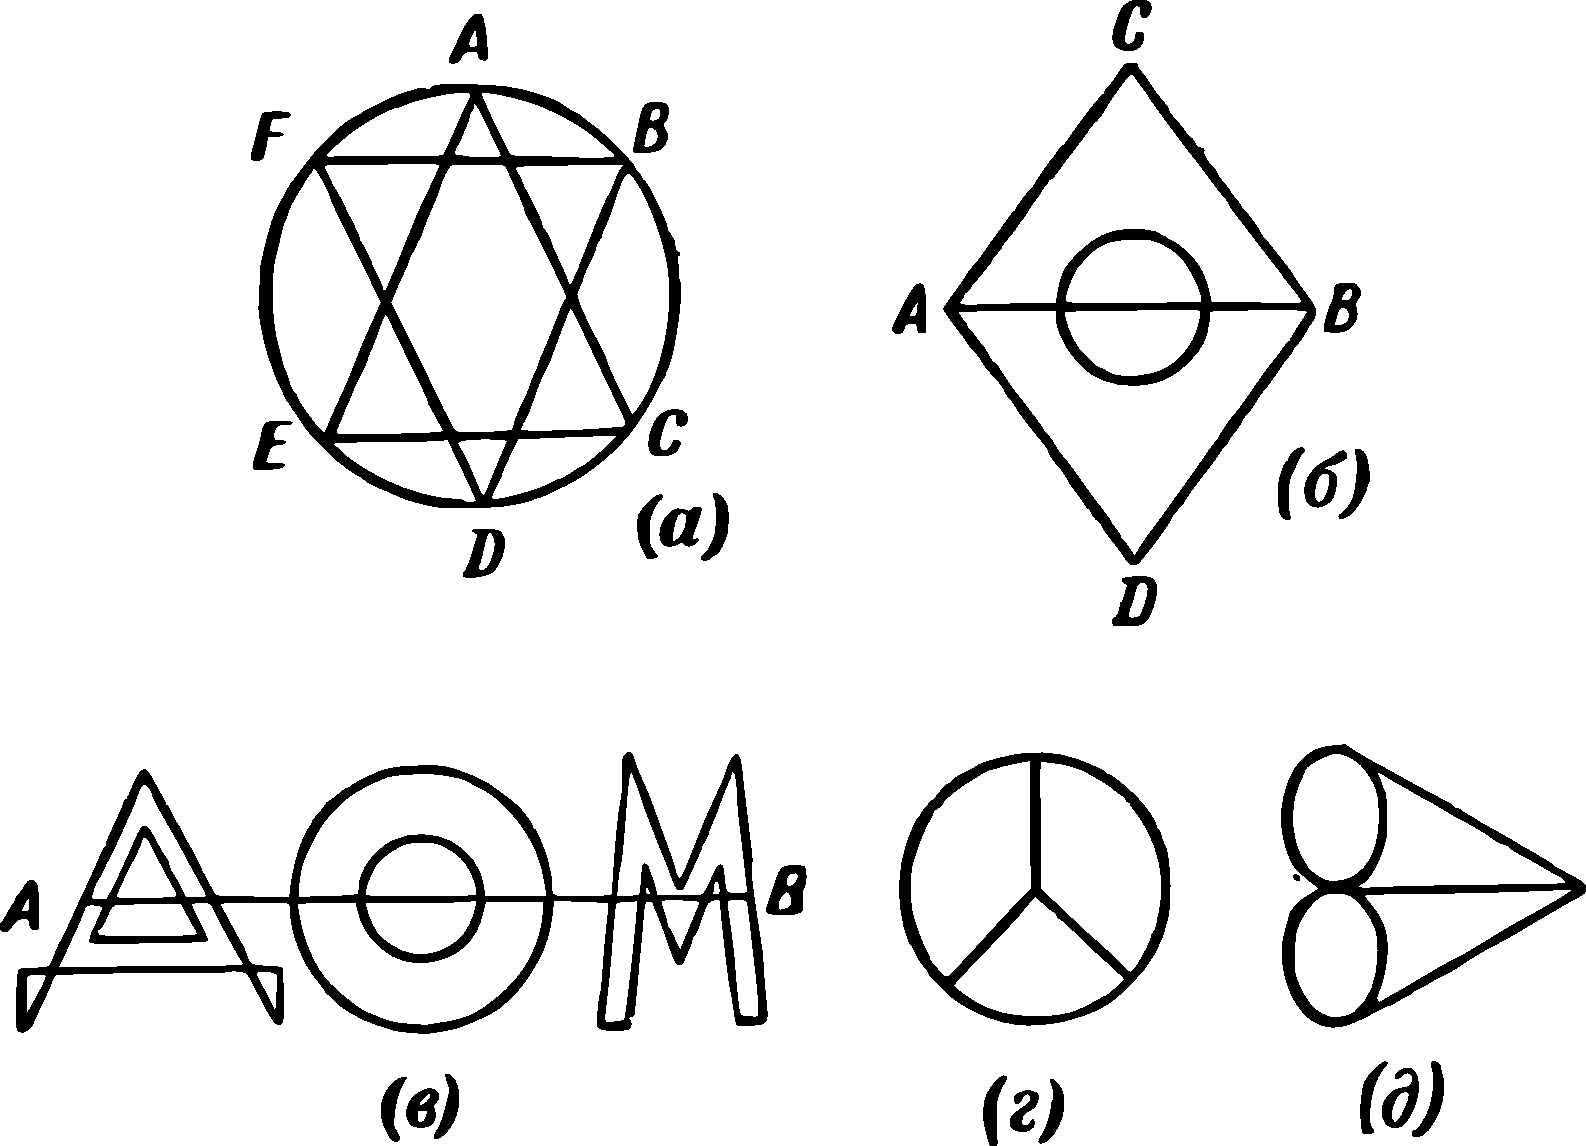
\includegraphics[width=0.9\textwidth]{figures/ch-10/fig-155.pdf}
\sidecaption{Try to draw each shape with a single stroke, without drawing the same line more than once.\label{fig-155}}
\end{figure}


Many of those who were given this problem started with figure \emph{(d)}, as it appeared to be the simplest. However, all their attempts to draw this figure in one stroke failed. Disheartened, they approached the remaining figures with less confidence and, to their surprise and satisfaction, managed to solve the first two figures and even the intricate third one, which represents the crossed-out word $AOM$ \emph{(c)}, without much difficulty. But no one managed to trace the fifth figure \emph{(e)}, just like the fourth figure \emph{(d)}, in one stroke.

Why is it possible to solve the problem for some figures but not for others? Is it perhaps only because our ingenuity is lacking in some cases, or maybe the problem itself is generally unsolvable for certain figures? Is there any way to indicate a criterion that would allow us to determine in advance whether we can trace a given figure in one stroke or not?

\ans Let's call each intersection where the lines of a given figure meet a node. We will call a node even if an even number of lines meet at that point, and odd if an odd number of lines meet there. In figure \emph{(a)}, all nodes are even; in figure \emph{(b)}, there are two odd nodes (points $A$ and $B$); in figure \emph{(c)}, the ends of the segment crossing out the word $AOM$ are odd nodes; in figures \emph{(d)} and \emph{(e)}, there are four odd nodes each.

Let's first consider a figure in which all nodes are even, such as figure \emph{(a)}. We start our path from any point $S$. Passing through node $A$, for example, we draw two lines: one leading to $A$ and one leading out from $A$. Since each even node has as many exits as it has entrances, as we move from node to node, the number of unmarked lines decreases by two each time. Therefore, in principle, it is quite possible to return to the starting point $S$ after traversing all the lines.

But suppose we return to the starting point and there are no more exits from it, yet there is still an unmarked line on the figure, originating from some node $B$ that we have already visited. This means we need to adjust our path: upon reaching node $B$, we first need to mark the missed lines and, returning to $B$, continue along the original path.

For example, let's say we decide to traverse figure \emph{(a)} as follows: first along the sides of the triangle $ACE$, then, returning to point $A$, along the perimeter $ABCDEFA$ (see \figr{fig-155}). Since this leaves the triangle $BDF$ unmarked, before we leave node $B$ and proceed along arc $BC$, we should first traverse triangle $BDF$.

Therefore, if all nodes of a given figure are even, then starting from any point in the figure, it is always possible to mark the entire figure with a single stroke. In this case, the traversal of the figure should end at the same point from which it started.

Now, let's consider a figure that has two odd nodes.

Figure \emph{(b)}, for example, has two odd nodes $A$ and $B$.

It can also be traced with a single stroke.


In fact, let's start the detour from odd node \nom{1} and follow some line to odd node \nom{2}, for example, from $A$ to $B$ along the $ACB$ in figure \emph{(b)} (\figr{fig-155}).

By drawing this line, we thereby exclude one line from each odd node, as if this line did not exist in the figure. Both odd nodes then become even. Since there were no other so-called even nodes in the figure, now we have a figure with only even nodes; in figure \emph{(b)}, for example, after drawing the $ACB$ line, a triangle with a circle remains.

So, if the figure contains two odd nodes, then a successful stroke should start in one of them and end in the other.


One additional note: starting from the odd node \nom{1}, it is necessary to choose the path leading to the odd node \nom{2} so that no figures isolated from this figure are formed. \sidenote{The inquisitive reader will find the details related to the issue under discussion in topology textbooks.}. For example, when drawing figure \emph{(b)} in \figr{fig-155}, it would be unsuccessful to hurry from the odd node $A$ to the odd node $B$ in a straight line $AB$, since in this case the circle would remain isolated from the rest of the figure and not drawn.

So, if the figure contains two odd nodes, then a successful stroke should start at one of them and end at the other.

Thus, the ends of the stroke are separated.

From here, it follows in turn that if a figure has four odd nodes, then it can be traced not with one stroke, but with two, but this no longer corresponds to the condition of our problem. Such are, for example, figures \emph{(d)} and \emph{(e)} in \figr{fig-155}.

As you can see, if one learns to reason correctly, much can be anticipated, thereby saving oneself from unnecessary expenditure of effort and time, and correct reasoning teaches, among other things, geometry.

Perhaps, dear reader, you may have found the reasoning presented here somewhat tiresome, but your efforts are rewarded by the advantage that knowledge brings over ignorance.

\begin{figure}[h!]
\centering
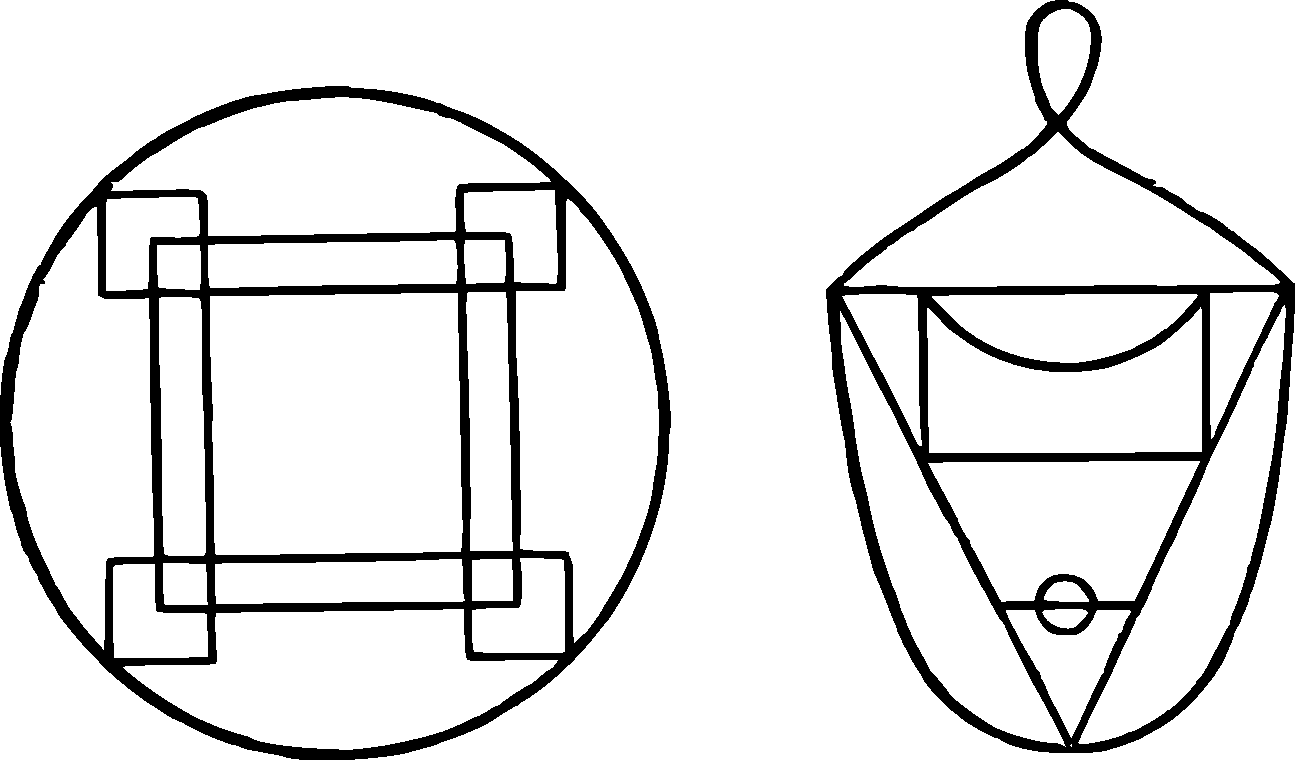
\includegraphics[width=0.7\textwidth]{figures/ch-10/fig-156.pdf}
\sidecaption{Draw each shape with a single stroke.\label{fig-156}}
\end{figure}


You can always determine in advance whether the task of traversing a given figure is solvable and know from which node to start its traversal.

Moreover, you can now easily come up with as many as you want intricate figures of this kind for your friends. As a conclusion, draw a couple more figures depicted in \figr{fig-156}.


\section{The Seven Bridges of K\"onigsberg}
\label{sec-10.10}

Two hundred years ago, in the city of K\"onigsberg\sidenote{At that time it was called K\"onigsberg.}, there were seven bridges connecting the banks of the Pregel River (see \figr{fig-157}).


\begin{figure}[h!]
\centering
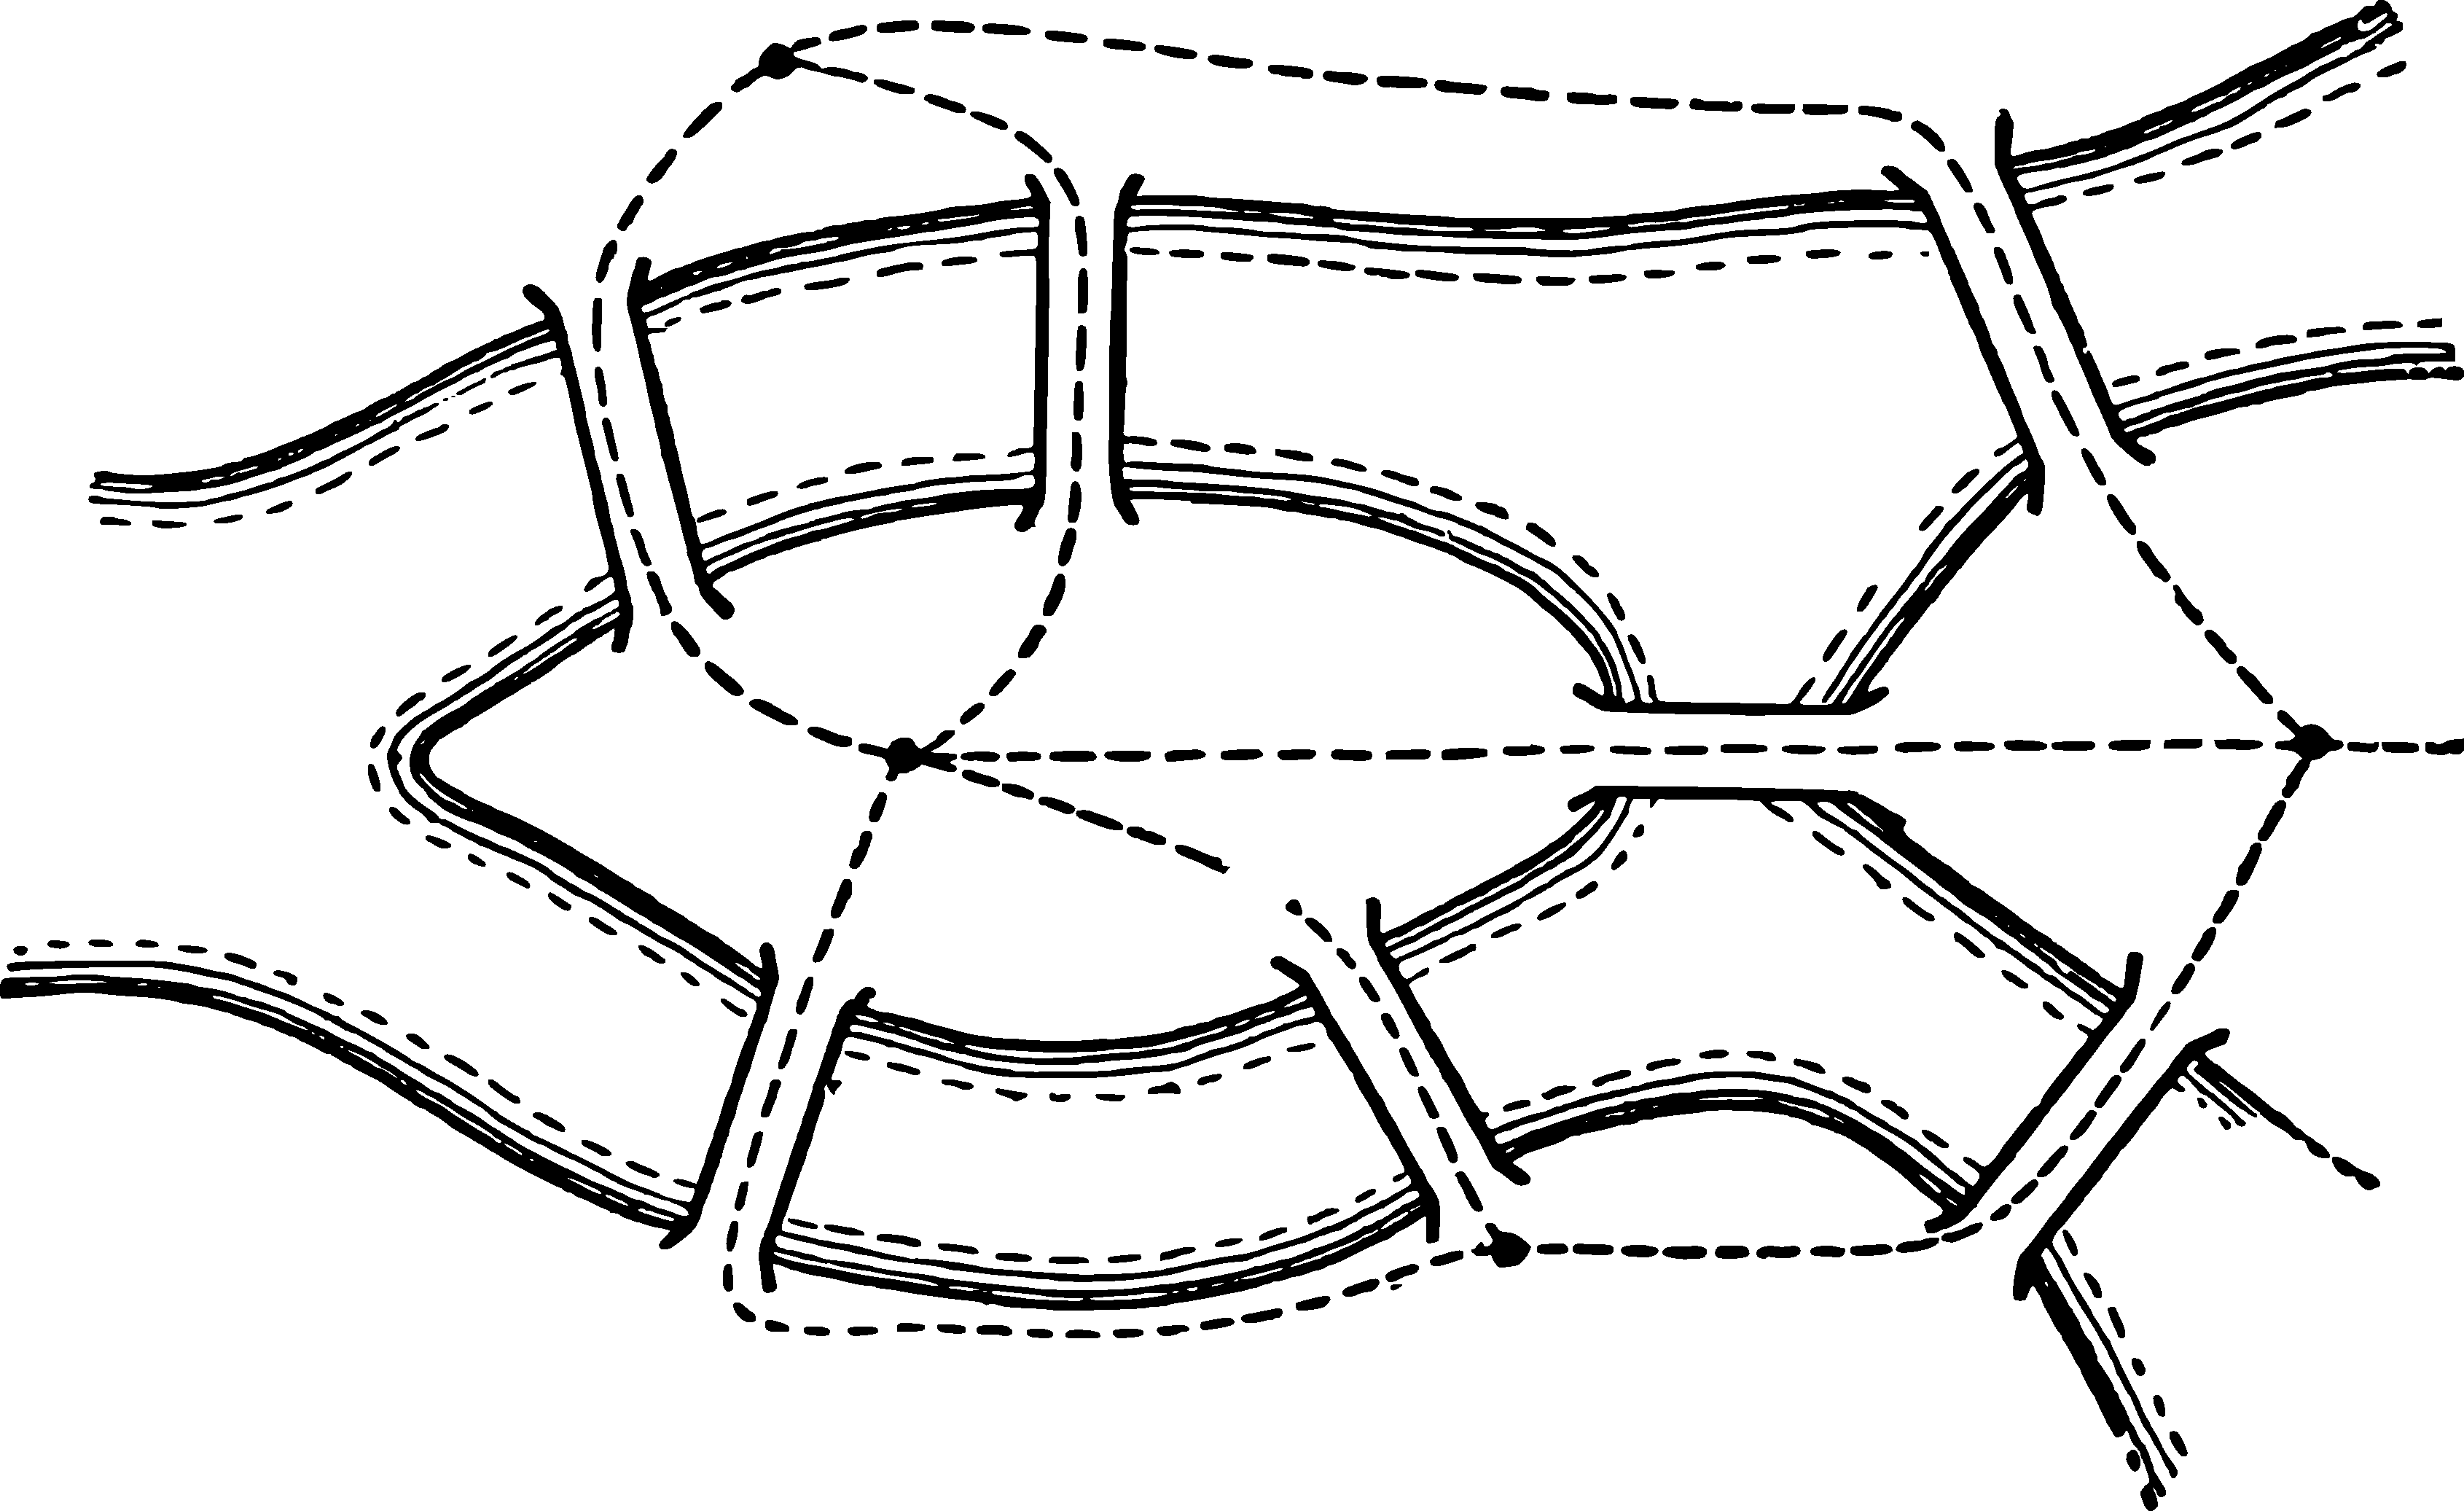
\includegraphics[width=0.9\textwidth]{figures/ch-10/fig-157.pdf}
\sidecaption{Is it possible to cross all these seven bridges, having visited each of them only once?\label{fig-157}}
\end{figure}


In 1736, the eminent mathematician of the time, Leonhard Euler (then around 30 years old), became interested in the following question: is it possible, while strolling through the city, to cross all seven bridges, but each only once?

It is easy to see that this problem is equivalent to the recently discussed problem of tracing a figure.

Let's depict the possible paths (dotted lines in \figr{fig-157}). It turns out to be one of the figures from the previous problem with four odd nodes (see \figr{fig-155}, figure \emph{(e)}). As you now know, it cannot be traced with a single stroke, and therefore, it is impossible to cross all seven bridges, passing over each of them only once. Euler then proved this.



\section{Geometrical Joke}
\label{sec-10.11}

After you and your companions have learned the secret of successfully tracing a figure with a single stroke, announce to your friends that you are still willing to draw a figure with four odd nodes, for example, a circle with two diameters (see \figr{fig-158}), without lifting the pencil from the paper and without tracing any line twice.

You know perfectly well that this is impossible, but you can insist on your sensational statement. Let me now teach you a little trick.

\begin{figure}[h!]
\centering
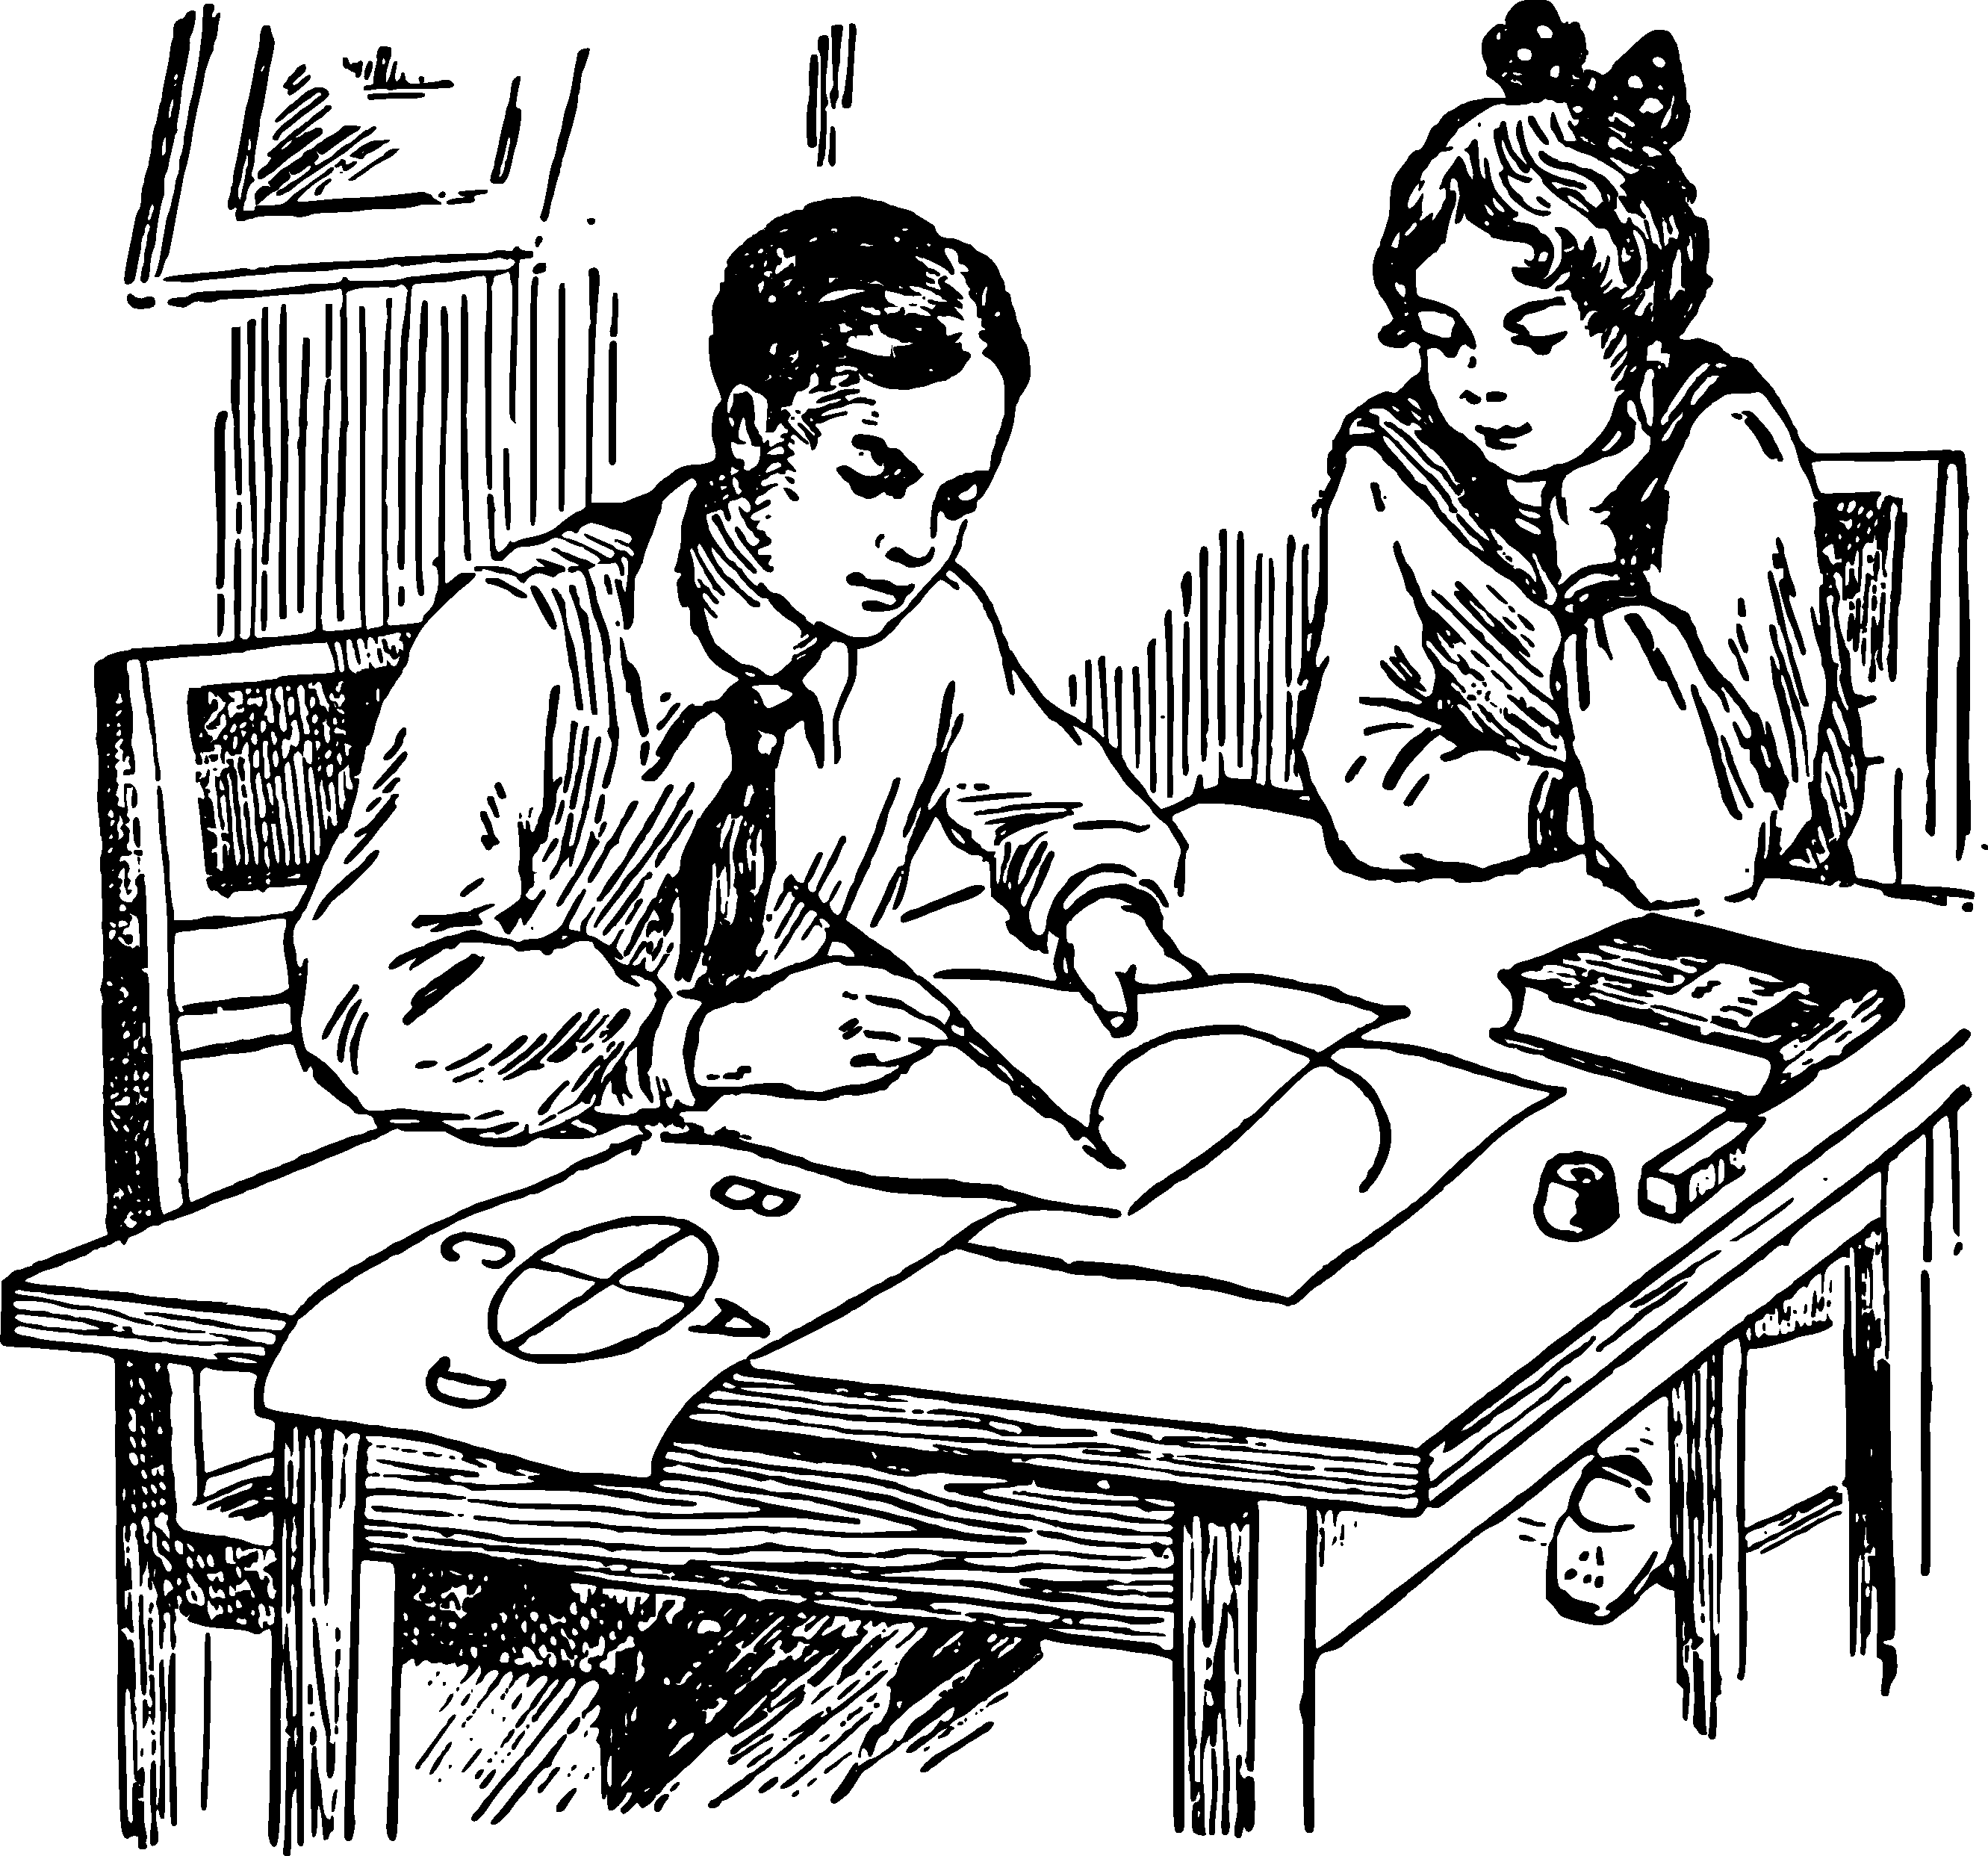
\includegraphics[width=0.9\textwidth]{figures/ch-10/fig-158.pdf}
\sidecaption{Geometric joke.\label{fig-158}}
\end{figure}



Start drawing the circle from point $A$ (\figr{fig-158}). As soon as you draw a quarter of the circle -- arc $AB$, place another sheet of paper at point $B$ (or fold the bottom part of the sheet on which you are making the construction) and continue tracing the lower part of the semicircle to point $D$, opposite point $B$.

Now remove the placed piece of paper (or unfold your sheet). On the front side of your sheet of paper, only the arc $AB$ will be drawn, but the pencil will be at point $D$ (even though you did not lift it from the paper!).

It's easy to complete the figure: first draw arc $DA$, then diameter $AC$, arc $CD$, diameter $DB$, and finally arc $BC$. You can also choose another route from point $D$; find it.


\section{Form Verification Problem}
\label{sec-10.12}

\ques Wanting to check whether a cut piece of fabric has the shape of a square, a seamstress ensures that when folding along the diagonals, the edges of the fabric coincide. Is this check sufficient?

\ans By this method, the seamstress only ensures that all sides of the quadrilateral piece of fabric are equal. Not only does a square possess this property among convex quadrilaterals, but also any rhombus, and a rhombus represents a square only when its angles are right angles. Therefore, the check applied by the seamstress is insufficient. It is necessary to visually confirm at least that the angles at the vertexes of the piece of fabric are right angles. For this purpose, for example, the piece can be additionally folded along its median line and the angles adjacent to one side can be observed to coincide.

\section{Game}
\label{sec-10.13}

For the game, a rectangular sheet of paper and figures of identical and symmetrical shapes are needed, such as dominoes or coins of equal value, or matchboxes, etc. The number of figures should be sufficient to cover the entire sheet of paper. Two players participate. Players take turns placing figures in any position on any free space on the sheet of paper until they have nowhere left to place them.

It is not allowed to move the placed figures on the paper. The player who places the item last is considered the winner.



\ques Find a way to conduct the game in which the player who starts always wins.



\ans The player starting the game should, on their first move, occupy the central area of the sheet by placing their figure in such a way that its centre of symmetry, if possible, coincides with the centre of the sheet of paper. They should then continue to place their figure symmetrically to the opponent's figure (see \figr{fig-159}).


\begin{figure}[h!]
\centering
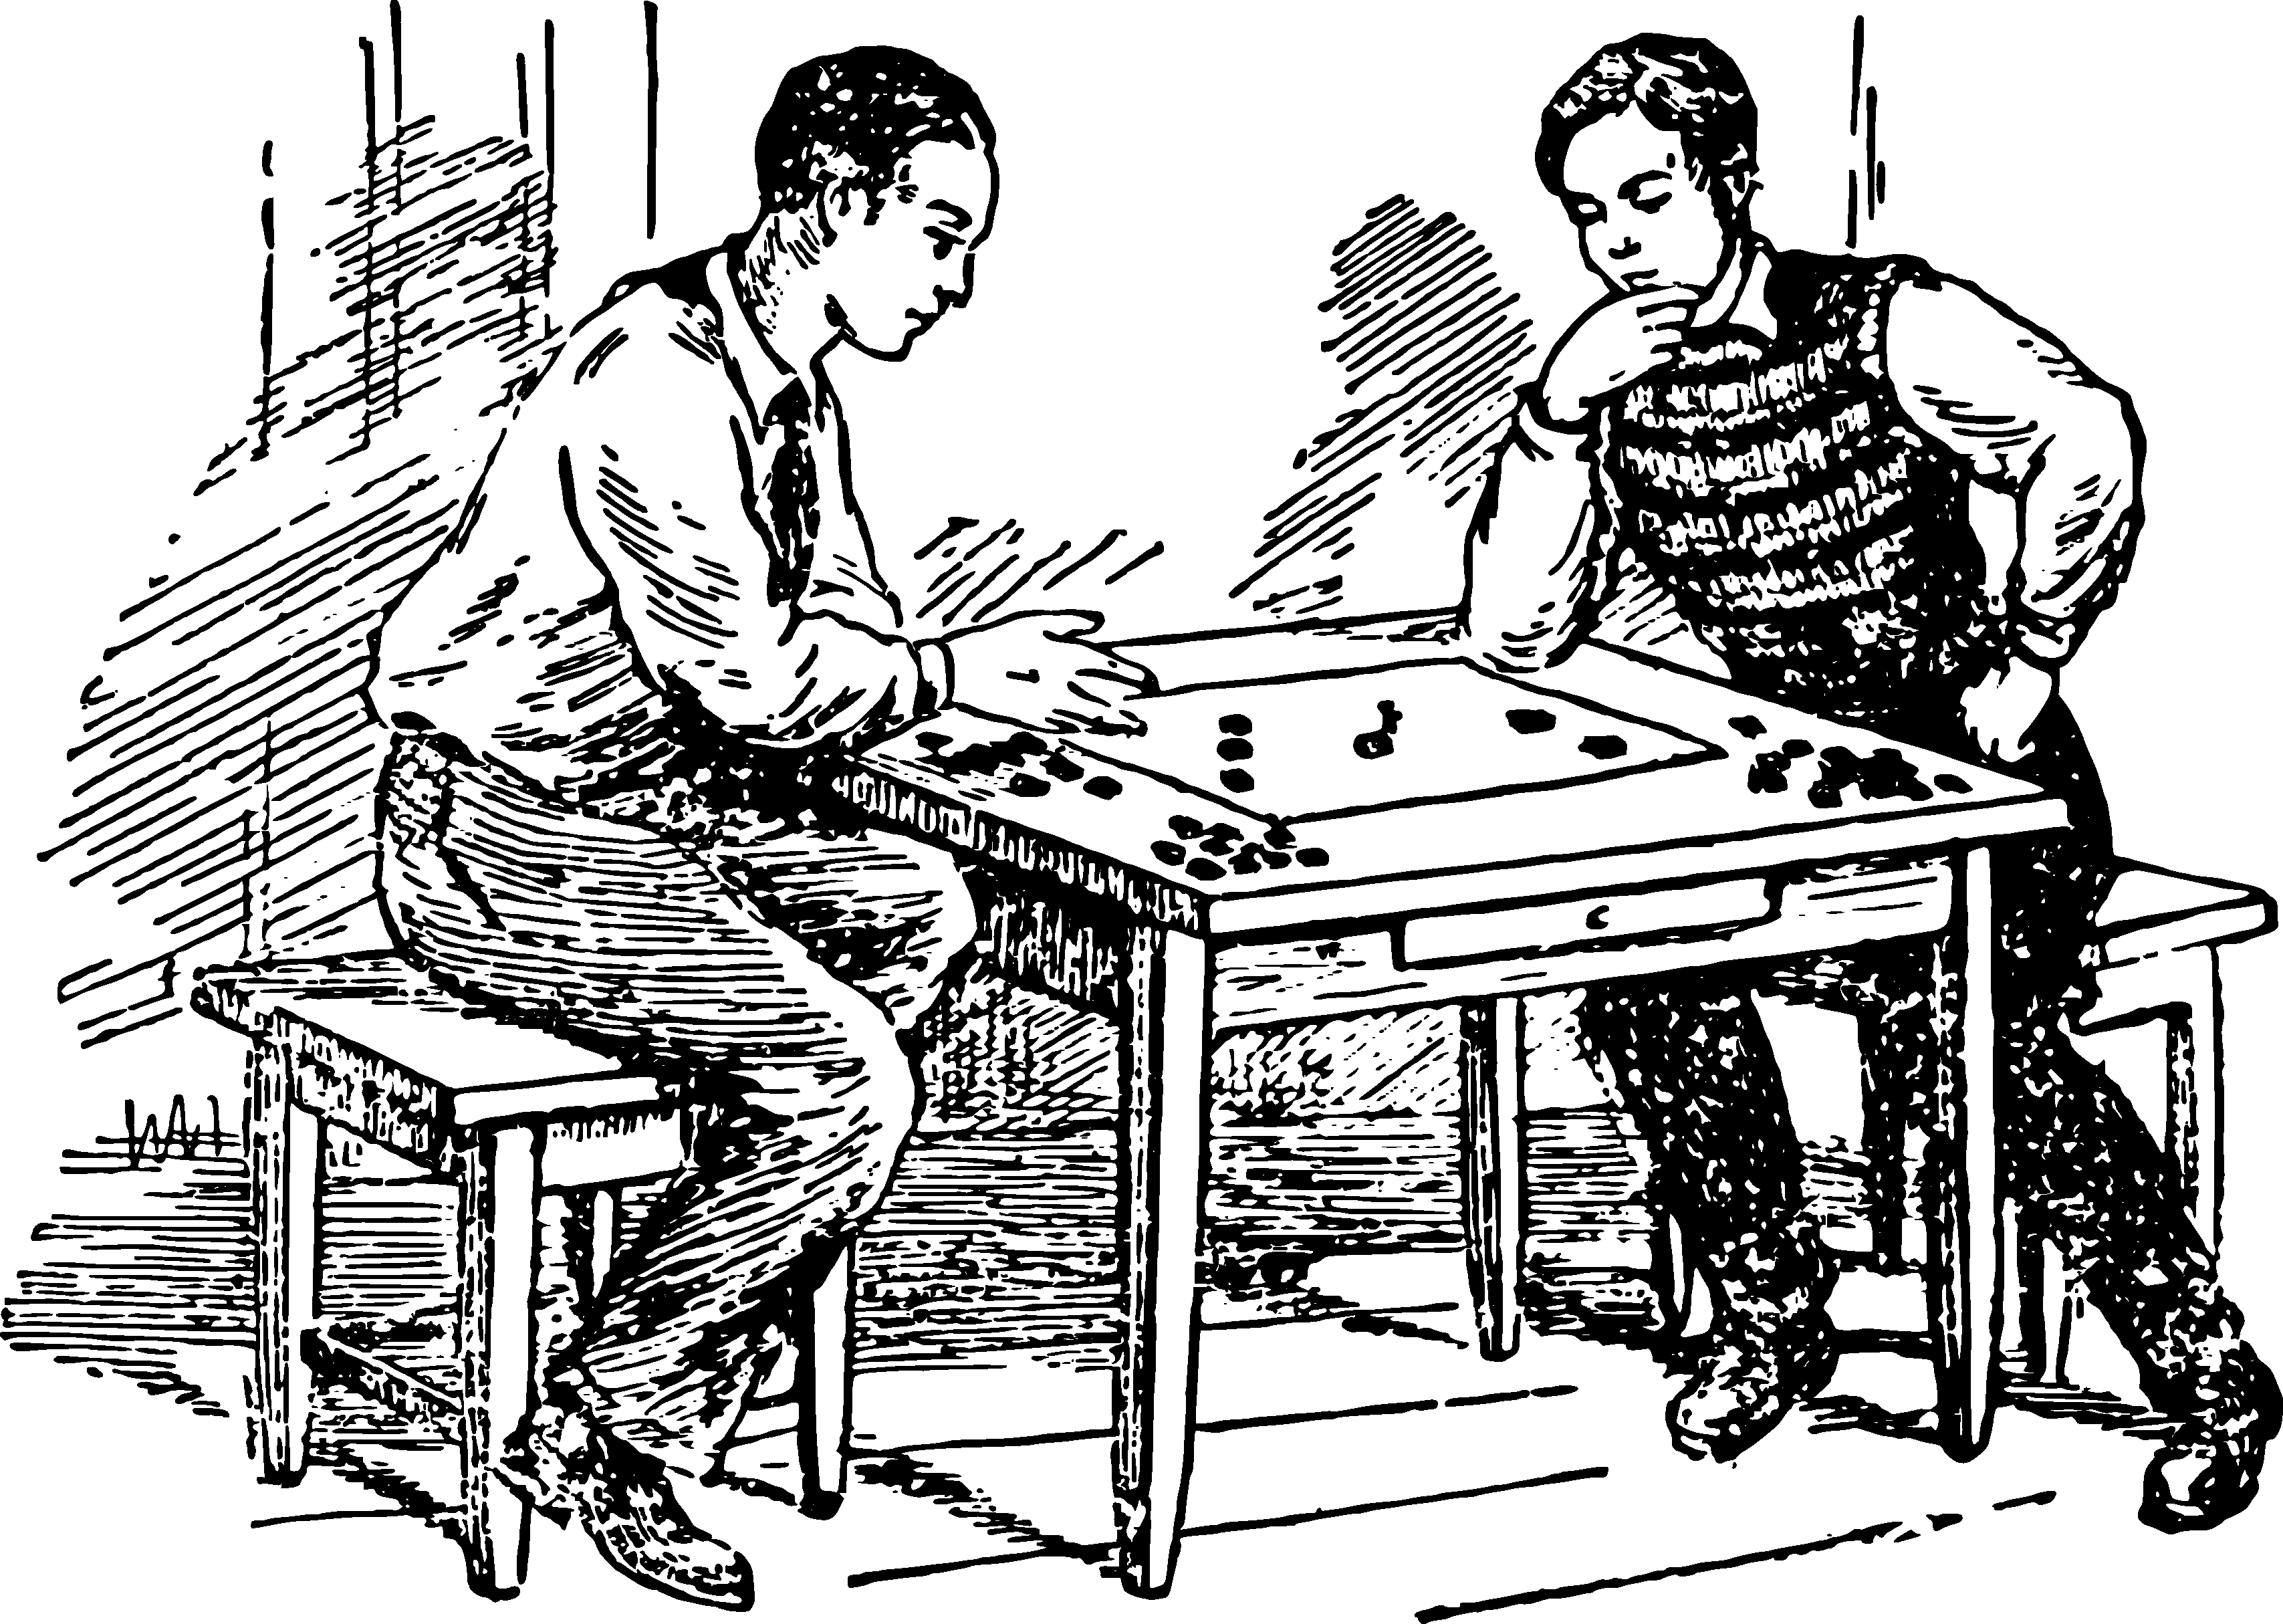
\includegraphics[width=0.9\textwidth]{figures/ch-10/fig-159.pdf}
\sidecaption{Geometric game. The winner is the one who places the item last.\label{fig-159}}
\end{figure}


Adhering to this rule, the player who starts the game will always find a place for their figure on the sheet of paper and will inevitably win.

The geometric essence of the mentioned way of conducting the game is as follows: a rectangle has a centre of symmetry, i.e., a point at which all straight line segments passing through it are divided in half and divide the figure into two equal parts. Therefore, every point or area of the rectangle corresponds to a symmetric point or area belonging to the same figure, and only the centre of the rectangle does not have a symmetric point.

From this, it follows that if the first player occupies the central area, then, no matter where the opponent chooses to place their figure, there will always be a free area on the rectangular sheet of paper that is symmetric to the area occupied by the opponent's figure.

Since the second player has to choose a place for their figure each time, eventually there will be no space left on the paper specifically for their figures, and the first player will win the game.

\begin{center}
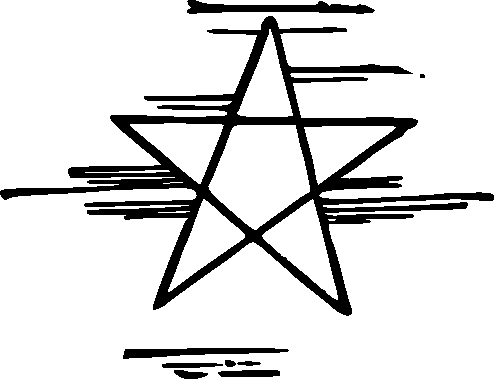
\includegraphics[width=0.3\textwidth]{figures/ch-10/fig-ch-10-tail.pdf}
\end{center}


















